%==============================================================================
% tento soubor pouzijte jako zaklad
% this file should be used as a base for the thesis
% Autoři / Authors: 2008 Michal Bidlo, 2016 Jaroslav Dytrych
% Kontakt pro dotazy a připomínky: dytrych@fit.vutbr.cz
% Contact for questions and comments: dytrych@fit.vutbr.cz
%==============================================================================
% kodovaní: UTF-8 (zmena prikazem iconv, recode nebo cstocs)
% encoding: UTF-8 (you can change it by command iconv, recode or cstocs)
%------------------------------------------------------------------------------
% zpracování / processing: make, make pdf, make clean
%==============================================================================
% Soubory, které je nutné upravit: / Files which have to be edited:
%   projekt-20-literatura-bibliography.bib - literatura / bibliography
%   projekt-01-kapitoly-chapters.tex - obsah práce / the thesis content
%   projekt-30-prilohy-appendices.tex - přílohy / appendices
%==============================================================================
%\documentclass[]{fitthesis} % bez zadání - pro začátek práce, aby nebyl problém s překladem
%\documentclass[english]{fitthesis} % without assignment - for the work start to avoid compilation problem
\documentclass[zadani]{fitthesis} % odevzdani do wisu - odkazy jsou barevné
%\documentclass[english,zadani]{fitthesis} % for submission to the IS FIT - links are color
%\documentclass[zadani,print]{fitthesis} % pro tisk - odkazy jsou černé
%\documentclass[zadani,cprint]{fitthesis} % pro barevný tisk - odkazy jsou černé, znak VUT barevný
%\documentclass[english,zadani,print]{fitthesis} % for the color print - links are black
%\documentclass[english,zadani,cprint]{fitthesis} % for the print - links are black, logo is color
% * Je-li prace psana v anglickem jazyce, je zapotrebi u tridy pouzit 
%   parametr english nasledovne:
%   If thesis is written in english, it is necessary to use 
%   parameter english as follows:
%      \documentclass[english]{fitthesis}
% * Je-li prace psana ve slovenskem jazyce, je zapotrebi u tridy pouzit 
%   parametr slovak nasledovne:
%      \documentclass[slovak]{fitthesis}

% Základní balíčky jsou dole v souboru šablony fitthesis.cls
% Basic packages are at the bottom of template file fitthesis.cls
%zde muzeme vlozit vlastni balicky / you can place own packages here

%---rm---------------
\renewcommand{\rmdefault}{lmr}%zavede Latin Modern Roman jako rm / set Latin Modern Roman as rm
%---sf---------------
\renewcommand{\sfdefault}{qhv}%zavede TeX Gyre Heros jako sf
%---tt------------
\renewcommand{\ttdefault}{lmtt}% zavede Latin Modern tt jako tt

% vypne funkci šablony, která automaticky nahrazuje uvozovky,
% aby nebyly prováděny nevhodné náhrady v popisech API apod.
% disables function of the template which replaces quotation marks
% to avoid unnecessary replacements in the API descriptions etc.
\csdoublequotesoff

% =======================================================================
% balíček "hyperref" vytváří klikací odkazy v pdf, pokud tedy použijeme pdflatex
% problém je, že balíček hyperref musí být uveden jako poslední, takže nemůže
% být v šabloně
% "hyperref" package create clickable links in pdf if you are using pdflatex.
% Problem is that this package have to be introduced as the last one so it 
% can not be placed in the template file.
\ifWis
\ifx\pdfoutput\undefined % nejedeme pod pdflatexem / we are not using pdflatex
\else
  \usepackage{color}
  \usepackage[unicode,colorlinks,hyperindex,plainpages=false,pdftex]{hyperref}
  \definecolor{links}{rgb}{0.4,0.5,0}
  \definecolor{anchors}{rgb}{1,0,0}
  \def\AnchorColor{anchors}
  \def\LinkColor{links}
  \def\pdfBorderAttrs{/Border [0 0 0] }  % bez okrajů kolem odkazů / without margins around links
  \pdfcompresslevel=9
\fi
\else % pro tisk budou odkazy, na které se dá klikat, černé / for the print clickable links will be black
\ifx\pdfoutput\undefined % nejedeme pod pdflatexem / we are not using pdflatex
\else
  \usepackage{color}
  \usepackage[unicode,colorlinks,hyperindex,plainpages=false,pdftex,urlcolor=black,linkcolor=black,citecolor=black]{hyperref}
  \definecolor{links}{rgb}{0,0,0}
  \definecolor{anchors}{rgb}{0,0,0}
  \def\AnchorColor{anchors}
  \def\LinkColor{links}
  \def\pdfBorderAttrs{/Border [0 0 0] } % bez okrajů kolem odkazů / without margins around links
  \pdfcompresslevel=9
\fi
\fi
% Řešení problému, kdy klikací odkazy na obrázky vedou za obrázek
% This solves the problems with links which leads after the picture
\usepackage[all]{hypcap}

% Informace o práci/projektu / Information about the thesis
%---------------------------------------------------------------------------
\projectinfo{
  %Prace / Thesis
  project=DP,            %typ prace BP/SP/DP/DR  / thesis type (SP = term project)
  year=2018,             %rok odevzdání / year of submission
  date=\today,           %datum odevzdani / submission date
  %Nazev prace / thesis title
  title.cs={Distribuovaný repositář digitálních\\ forenzních dat},  %nazev prace v cestine ci slovenstine (dle zadani) / thesis title in czech language (according to assignment)
  title.en={Distributed Forensic Digital Data Repository}, %nazev prace v anglictine / thesis title in english
  %Autor / Author
  author={Martin Josefík},   %cele jmeno a prijmeni autora / full name and surname of the author
  author.name={Martin},   %jmeno autora (pro citaci) / author name (for reference) 
  author.surname={Josefík},   %prijmeni autora (pro citaci) / author surname (for reference) 
  author.title.p=Bc., %titul pred jmenem (nepovinne) / title before the name (optional)
  %author.title.a=PhD, %titul za jmenem (nepovinne) / title after the name (optional)
  %Ustav / Department
  department=UIFS, % doplnte prislusnou zkratku dle ustavu na zadani: UPSY/UIFS/UITS/UPGM
  %                  fill in appropriate abbreviation of the department according to assignment: UPSY/UIFS/UITS/UPGM
  %Skolitel / supervisor
  supervisor=Marek Rychlý, %cele jmeno a prijmeni skolitele / full name and surname of the supervisor
  supervisor.name={Marek},   %jmeno skolitele (pro citaci) / supervisor name (for reference) 
  supervisor.surname={Rychlý},   %prijmeni skolitele (pro citaci) / supervisor surname (for reference) 
  supervisor.title.p=RNDr.,   %titul pred jmenem (nepovinne) / title before the name (optional)
  supervisor.title.a={Ph.D.},    %titul za jmenem (nepovinne) / title after the name (optional)
  %Klicova slova, abstrakty, prohlaseni a podekovani je mozne definovat 
  %bud pomoci nasledujicich parametru nebo pomoci vyhrazenych maker (viz dale)
  %Keywords, abstracts, declaration and acknowledgement can be defined by following 
  %parameters or using dedicated macros (see below)
  %===========================================================================
  %Klicova slova / keywords
  %keywords.cs={Klíčová slova v českém jazyce.}, %klicova slova v ceskem ci slovenskem jazyce
  %                                              keywords in czech or slovak language
  %keywords.en={Klíčová slova v anglickém jazyce.}, %klicova slova v anglickem jazyce / keywords in english
  %Abstract
  %abstract.cs={Výtah (abstrakt) práce v českém jazyce.}, % abstrakt v ceskem ci slovenskem jazyce
  %                                                         abstract in czech or slovak language
  %abstract.en={Výtah (abstrakt) práce v anglickém jazyce.}, % abstrakt v anglickem jazyce / abstract in english
  %Prohlaseni / Declaration
  %declaration={Prohlašuji, že jsem tuto bakalářskou práci vypracoval samostatně pod vedením pana ...},
  %Podekovani (nepovinne) / Acknowledgement (optional)
  %acknowledgment={Zde je možné uvést poděkování vedoucímu práce a těm, kteří poskytli odbornou pomoc.} % nepovinne
  %acknowledgment={Here it is possible to express thanks to the supervisor and to the people which provided professional help.} % optional
}

%Abstrakt (cesky, slovensky ci anglicky) / Abstract (in czech, slovak or english)
\abstract[cs]{Tato práce se zabývá návrhem distribuovaného repositáře zaměřeného jako úložiště rozsáhlých digitálních forenzních dat. Teoretická část práce pojednává o~forenzní analýze digitálních dat a~co je jejím cílem. Současně také vysvětluje Big data, vhodné úložiště, jejich vlastnosti, výhody a~nevýhody.
Hlavní část práce se pak zabývá návrhem a~implementací distribuovaného úložiště pro digitální forenzní data. Návrh se rovněž zaměřuje na vhodnou indexaci uložených dat a~rozšiřitelnost pro podporu nových druhů digitálních forenzních dat do budoucna.
Implementovaný systém byl otestován z~hlediska výkonnosti pro vstupní data PCAP soubory.
}

\abstract[en]{This work deals with the design of distributed repository aimed at storing digital forensic data. The theoretical part of the thesis describes digital forensics and what is its purpose. There are also explained Big data, suitable storages, their properties, advantages and disadvantages, in this part.
The main part of the thesis deals with the design and implementation of distributed storage for digital forensic data. The design is also focused in suitable indexing of stored data, and supporting new types of digital forensic data.
The performance of implemented system was evaluated for chosen type of digital forensic data PCAP files.
}

%Klicova slova (cesky, slovensky ci anglicky) / Keywords (in czech, slovak or english)
\keywords[cs]{Big data, forenzní analýza digitálních dat, formáty digitálních forenzních dat, AFF4, distribuované databáze, NoSQL databáze, Big data technologie, Kafka, asynchronní komunikace, reaktivní paradigma, Hadoop, HDFS, Cassandra, MongoDB, Spring Boot, PCAP soubory}

\keywords[en]{Big data, digital forensics, forensics file formats, AFF4, distributed databases, NoSQL databases, Big data technologies, Kafka, asynchronous communication, reactive programming, Hadoop, HDFS, Cassandra, MongoDB, Spring Boot, PCAP file}

%Prohlaseni (u anglicky psane prace anglicky, u slovensky psane prace slovensky)
%Declaration (for thesis in english should be in english)
\declaration{Prohlašuji, že jsem tuto diplomovou práci vypracoval samostatně pod vedením pana RNDr. Marka Rychlého, Ph.D. Uvedl jsem všechny literární prameny a~publikace, ze kterých jsem čerpal.}

%Podekovani (nepovinne, nejlepe v jazyce prace) / Acknowledgement (optional, ideally in the language of the thesis)
\acknowledgment{Rád bych touto cestou poděkoval vedoucímu mé diplomové práce panu RNDr. Markovi Rychlému, Ph.D. za odborné vedení, poskytované rady a~připomínky v~průběhu řešení práce.}

% řeší první/poslední řádek odstavce na předchozí/následující stránce
% solves first/last row of the paragraph on the previous/next page
\clubpenalty=10000
\widowpenalty=10000

\begin{document}
  % Vysazeni titulnich stran / Typesetting of the title pages
  % ----------------------------------------------
  \maketitle
  % Obsah
  % ----------------------------------------------
  \setlength{\parskip}{0pt}

  {\hypersetup{hidelinks}\tableofcontents}
  
  % Seznam obrazku a tabulek (pokud prace obsahuje velke mnozstvi obrazku, tak se to hodi)
  % List of figures and list of tables (if the thesis contains a lot of pictures, it is good)
  \ifczech
    \renewcommand\listfigurename{Seznam obrázků}
  \fi
  \ifslovak
    \renewcommand\listfigurename{Zoznam obrázkov}
  \fi
  % \listoffigures
  
  \ifczech
    \renewcommand\listtablename{Seznam tabulek}
  \fi
  \ifslovak
    \renewcommand\listtablename{Zoznam tabuliek}
  \fi
  % \listoftables 

  \ifODSAZ
    \setlength{\parskip}{0.5\bigskipamount}
  \else
    \setlength{\parskip}{0pt}
  \fi

  % vynechani stranky v oboustrannem rezimu
  % Skip the page in the two-sided mode
  \iftwoside
    \cleardoublepage
  \fi

  % Text prace / Thesis text
  % ----------------------------------------------
  %=========================================================================
% (c) Michal Bidlo, Bohuslav Křena, 2008


\chapter{Úvod}
Během začátku 21. století došlo k~ohromnému růstu v~oblastech internetu, sociálních sítí, multimédií, chytrých telefonů a~dalších digitálních zařízení, či mobilních plateb a~on-line transakcí. V~podstatě ve všech oblastech jako je například věda, politika, strojírenství, medicína, doprava, energetika, se nevyhneme použití digitálních zařízení. S~tím velmi úzce souvisí nárůst objemu digitálních dat, která je potřeba ukládat, analyzovat, zpracovávat, a~také vyšetřovat.

Digitální zařízení se mohou stát terčem útoků, může se jednat o~krádež citlivých dat, podvržení dat, sledování a~další. Digitální zařízení mohou být také nástrojem zločinu.

Rozdílnost mezi formáty digitálních dat, jejich strukturované a~nestrukturované vlastnosti, a~také prudký nárůst vyžadují mnoho rozličných přístupů a~technologií pro jejich zpracování.

Cílem této práce je navrhnout a~vytvořit distribuované úložiště pro digitální forenzní data. V~rámci teoretické části práce, se kapitola \ref{chapter1} zaměřuje na forenzní analýzu digitálních dat, vysvětluje, jak probíhá a~co je jejím cílem. Zabývá se také formáty digitálních forenzních dat a~existujícími systémy, které slouží k~uchování těchto dat a~důkazního materiálu. Následně je představen systém AFF4.

Kapitola \ref{chapter2} pojednává o~úložištích pro rozsáhlá strukturovaná i~nestrukturovaná data. V~jejich kontextu vysvětluje také termín Big data. Následují odstavce zaměřeny na distribuované databáze včetně jejich výhod a~nevýhod. Kapitola je završena uvedením principů NoSQL databází, rozdělení podle typů, a~srovnání s~relačními databázemi. Na NoSQL databázích bude založeno úložiště distribuovaného repositáře.

Cílem praktické části práce je navrhnout a~implementovat distribuovaný repositář. V~kapitole návrhu \ref{distrRepDesignChapter} je vysvětlena architektura systému, aplikační rozhraní, vlastnosti úložišť, princip ovládání repositáře a~také rozšiřitelnost pro nové druhy digitálních forenzních dat. Systém využívá Big data technologie. Pro komunikaci s~klientem jsou zprávy přenášeny tzv. \texttt{Message brokerem} Kafka. Jako úložiště slouží, v~závislosti na tom, o~jaký typ forenzních digitálních dat se jedná, NoSQL databáze a~distribuovaný souborový systém HDFS.

Kapitola \ref{chapter_impl} se zabývá implementací distribuovaného úložiště,  technickými detaily, způsobem asynchronní komunikace s~databázemi, ukládáním a~dotazováním nad daty (sekvenčním i~náhodným). Systém pracuje nad frameworkem Spring, který usnadňuje konfiguraci a~použití Big data komponent. Jako běhové prostředí byl zvolen projekt \texttt{Docker}, který poskytuje jednotné rozhraní pro izolaci aplikací do kontejnerů.

Poslední kapitola \ref{chapter_performance} se věnuje výkonnosti systému, hardwarovým požadavkům a~konfiguraci, a~použití systému pro vybrané druhy digitálních forenzních dat.

%Pro ověření základních aspektů návrhu byl také implementován prototyp distribuovaného repositáře, který řeší převážně rozhraní komunikace s~klientem, způsob ovládání repositáře, a~rovněž zpracování požadavků od klienta. Prototypem se zabývá kapitola \ref{chapterPrototype}.

\chapter{Forenzní analýza digitálních dat} \label{chapter1}
Forenzní analýza digitálních dat je věda identifikující, zachovávající, obnovující, analyzující a~předávající fakta ohledně digitálních důkazů nalezených v~počítačích nebo digitálních úložištích mediálních zařízení.
Nezabývá se tedy pouze počítači, ale také ostatními digitálními technologiemi včetně mobilních telefonů a~tabletů, mobilních sítí, internetového bankovnictví, datových médií apod.

Forenzní analýza digitálních dat slouží k~získání digitálního důkazního materiálu, který může být použit v~soudní síni proti obviněnému. Nalezené výstupy nejsou omezeny k~použití pouze u~soudu. Častokrát může nějaká firma řešit interní záležitosti jako například porušení firemní politiky, kdy se zase musí najít (digitální) důkaz, který potvrzuje nebo vyvrací obvinění.

Pod výše uvedenými aktivitami se skrývá \cite{whatIsDigFor}:

\begin{itemize}
\item Identifikace -- Jedná se o~první část celého procesu. Předtím, než je cokoliv zkoumáno a~analyzováno, je důležité identifikovat, kde jsou data uložena. Typicky jsou uložena na diskových jednotkách, serverech, flash klíčenkách, síťových zařízeních.

\item Zachování -- Důležitá je ochrana důkazů, tzn. pro sběr a~analýzu informací je potřeba zachovat původní data, musí se zabránit jejich změně a~ztrátě. Bez integrity je důkazní materiál nepoužitelný. Identifikovaná původní data mohou být zajištěna chronologickým řetězcem dokumentů (anglicky \texttt{chain of custody}), který zaznamenává veškeré aktivity s~digitálním důkazem jako je přenos, úschova, kontrola a~stav.

\item Obnovení -- Součástí procesu je i~obnova dat, která může zahrnovat obnovu smazaných dat procesy operačního systému, úmyslně smazané soubory, soubory chráněné heslem a~také poškozené soubory. I~po obnovení smazaného souboru musí být stále zachována integrita.

\item Analýza -- Jedná se o~hlavní část vyšetřování. Cílem je shromáždit co nejvíce relevantních artefaktů. Prohledávána je paměť, registry, výpisy z~logů aplikací, historie internetového prohlížeče apod. Podstatná je i~dokumentace všech kroků, které byly provedeny.

\item Předání -- Po analýze jsou artefakty důkladně zdokumentovány a~odevzdány například ve formě protokolu. Po shromáždění všech nalezených informací může ale nemusí dojít k~definitivnímu rozhodnutí. Co se s~informacemi stane už není v~rukou vyšetřovatele. Tady proces forenzní analýzy končí.
\end{itemize}

\noindent Vyšetřování digitálních forenzních dat obvykle zahrnuje vytvoření forenzní duplikace zkoumaného média. Provádí se proto, aby se neznehodnotil původní zdroj. Například dojde k~vytvoření obrazu disku, který je kopií celého disku nebo jeho části bit po bitu. Neduplikuje se celý systém, pokud je prostor příliš velký. Obraz je statický snímek, který může být analyzován za účelem odhalení nebo stanovení událostí ohledně incidentů, a~může tak být použitý jako důkaz v~soudní síni. Analýza je prováděna na kopii pro zachování integrity originálu.

Vyšetřovatel zanalyzuje obraz pomocí snímacích technik, aby získal relevantní data z~disku. Forenzní obraz obsahuje soubory z~disku, nealokovaný prostor a~tzv. \texttt{slack space}. Slack space je pozůstatek diskového prostoru, který byl alokován pro nějaký počítačový soubor a~ten všechen prostor nepotřebuje. Právě v~těchto prostorech mohou být nalezeny relevantní artefakty a~informace jako např. smazané soubory, či jejich fragmenty \cite{forensicImages}.

\begin{figure}[!h]
  \centering
  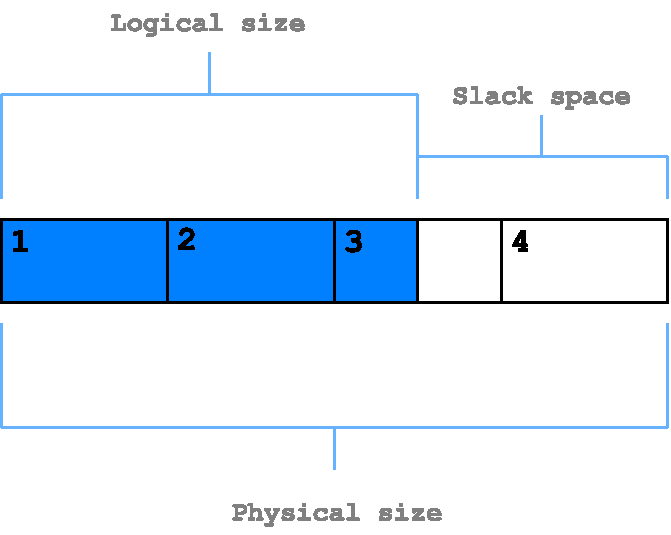
\includegraphics[width=10.5cm]{template-fig/SlackSpace.pdf}
  \caption{Příklad znázorňuje slack space pro parametry -- sektory velikosti 512 bajtů jsou shluknuty v~operačním systému do skupin po čtyřech, tzn. velikost svazku je 2048 bajtů; velikost souboru je 1280 bajtů (vyznačen modrou barvou). Pro tento soubor byl alokován celý svazek 2048 bajtů. Nevyužité místo (označeno bílou barvou) je slack space, v~tomto případě se jedná o~768 bajtů \cite{slacSpace}.}
  \label{FIG_SlackSpace}
\end{figure}

\section{Formáty digitálních forenzních dat}
Typů digitálních forenzních dat existuje spousta. Každý typ takových dat může být reprezentován jiným formátem. Tato sekce čerpá informace převážně z~\cite{forensicswikiForensicFF}.

Mnoho forenzních počítačových programů používá své vlastní formáty pro uložení informace. Můžeme je rozdělit na nezávislé (anglicky \texttt{Independent File Formats}) a~programově specifické formáty (anglicky \texttt{Program-Specific File Formats}):

\begin{itemize}
\item Nezávislé -- Tyto formáty byly vyvinuty nezávisle na konkrétním forenzním programu. Patří mezi ně \texttt{AFF}, \texttt{AFF4}, \texttt{gfzip}, \texttt{Raw Image Format}.

\item Programově specifické -- Byly vyvinuty pro použití specifickými forenzními programy. Většinou každý takový formát je unikátní, a~proto je pro přečtení potřeba unikátního nástroje.
Zástupci jsou například \texttt{Encase image file format}, \texttt{ProDiscover image file format}, \texttt{IXimager file formats}.
\end{itemize}

\subsubsection{Identifikace formátu}
%File Format Identification
Identifikace formátu souboru je proces určení formátu nějaké sekvence bajtů. Operační systém toto typicky dělá rozpoznáním přípony souboru nebo podle zabudované \texttt{MIME} informace. Forenzní aplikace musí identifikovat typy souborů podle obsahu. Mezi existující systémy patří například tyto projekty -- \texttt{libmagic}, \texttt{PRONOM}, \texttt{Apache Tika} \footnote{http://tika.apache.org/} \cite{forensicswikiFFIdentification}.

\section{Existující systémy}
Vyznamným zástupcem pro uložení digitálních forenzních dat je systém AFF4, který bude popsán detailněji.

\subsection{AFF4}
Jedná se o~open source formát pro ukládání digitálních důkazů a~dat. Jeho výhodami jsou správa metadat a~možnost komprese. Tato sekce čerpá převážně z~\cite{aff4}. Je založen na objektově orientované architektuře. Veškerá množina známých objektů je označována jako \texttt{AFF4 universe}. Takový prostor je definovaný jako nekonečný, protože AFF4 je navržen pro škálování obrovského množství důkazního materiálu. Všechny objekty jsou adresovatelné jejich jménem, které je v~rámci AFF4 universe unikátní.

\vspace{0.5cm}

\noindent Příkladem jména nějakého AFF4 objektu může být:

\texttt{urn:aff4:f3eba626-505a-4730-8216-1987853bc4d2}

\noindent Jedná se o~standardní URN notaci, URN je unikátní.

\vspace{0.5cm}

\noindent AFF4 universe používá RDF notaci pro specifikaci atributů objektů. V~nejjednodušší podobě je RDF množina tvrzení o~objektu ve formátu:

\texttt{Subject   Attribute   Value}

\vspace{0.5cm}

\noindent Příklad:

\noindent \texttt{******** Object urn:aff4:f3eba626-505a-4730-8216-1987853bc4d2 ***********}\\
\texttt{aff4:stored = urn:aff4:4bdbf8bc-d8a5-40cb-9af0-fd7e4d0e2c9e}\\
\texttt{aff4:type = image}\\
\texttt{aff4:interface = stream}\\
\texttt{aff4:timestamp = 0x49E9DEC3}\\
\texttt{aff4:chunk\_size = 32k}\\
\texttt{aff4:compression = 8}\\
\texttt{aff4:chunks\_in\_segment = 2048}\\
\texttt{aff4:size = 10485760}\\

\noindent Příklad ukazuje, že objekt má tyto atributy a~hodnoty. Nazýváme je relace nebo fakta. Celý AFF4 universe je sestavený z~takových faktů.

\noindent AFF4 objekty existují, protože dělají něco užitečného, což závisí na rozhraní, které představují. Aktuálně existuje několik rozhraní, nejvýznamnější jsou \texttt{Volume} a~\texttt{Stream}. Rozhraní objektu je fakt o~objektu, který nalezneme v~atributu \texttt{aff4:interface}.

\subsubsection{Rozhraní Volume}
Rozhraní Volume definujeme jako mechanismus ukládání, který dokáže uložit segment (bit binárních dat) pod nějaké jméno, a~získat jej podle tohoto jména. Aktuálně existují dvě implementace: \texttt{Directory} a~\texttt{ZipFile}.

\begin{itemize}
\item \texttt{Directory Volume} -- Tato implementace ukládá segmenty jako soubory uvnitř běžného adresáře v~souborovém systému. Hodí se zejména, pokud potřebujeme uložit obraz na souborový systém FAT, přičemž velikost segmentu je malá a~nenarazíme tak na omezení velikosti souboru. Je také možné založit adresář na nějaké HTTP adrese, což nám umožní používat obraz přímo z~webu.

\item \texttt{ZipFile Volume} -- Jak napovídá název, tato implementace ukládá segmenty uvnitř zip archivu. Malé soubory lze bez problémů otevřít obyčejným průzkumníkem (v~OS Windows např. \texttt{Windows Explorer}) a~data extrahovat. Zase je možné zapsat zip archiv přímo na HTTP server a~používat obraz přímo ze serveru.
\end{itemize}

\noindent Je možné převádět mezi oběma formáty z~jednoho na druhý, extrahovat zip archiv do adresáře a~nebo z~adresáře vytvořit zip archiv.

\subsubsection{Rozhraní Stream}
Streamy jsou základním rozhraním pro ukládání dat obrazu. Stream obsahuje metody typu \texttt{read}, \texttt{seek}, \texttt{tell} a~\texttt{close}. Podporuje ještě \texttt{write}, ale ne k~modifikaci obrazu, nýbrž k~jeho vytvoření (kvůli výše uvedené integritě zdroje). Pokud nějaký AFF4 objekt podporuje rozhraní stream, lze provést náhodné čtení jeho dat. Existuje několik specifických implementací rozhraní stream, některými z~nich jsou:

\begin{itemize}
\item \texttt{FileBackedObjects} -- Stream, který ukládá data v~souboru v~souborovém systému, jehož pozice je určena URN souboru.

\item \texttt{HTTPObject} -- Pozice souboru je udána pomocí URL. Objekt lze ukládat a~číst z~HTTP serveru. Implementace umožňuje přečíst určité rozmezí bajtů. Režie síťového provozu mezi klientem a~serverem je minimální. Je možné vyšetřit vzdálený obraz přes HTTP bez potřeby celé kopie obrazu. Z~důvodu bezpečnosti by měl být server pro zápis nějak omezen, například hesly, SSL certifikáty apod. Podpora čtení může být poskytnuta bez omezení, pokud je zdroj dat zašifrován. Zabezpečení serveru je ale mimo rozsah systému AFF4.

\item \texttt{Segments} -- Segmenty jsou komponenty uloženy přímo ve \texttt{Volume}. Volume je zjednodušeně řečeno objekt uchovávající segmenty. Segmenty by měly být použity pro malé streamy, protože prohledávat v~komprimovaných segmentech může být drahá operace. Segmenty jsou užitečné, pokud potřebujeme vytvořit logický obraz nějaké podmnožiny souborového systému (pouze některé soubory) a~ne forenzní obraz celkového systému.

\item \texttt{Image streams} -- Tyto streamy jsou opakem segmentů. Pro velké obrazy nemůžeme použít segmenty, protože by nebyly zkomprimovány efektivně. Image stream ukládá obraz v~tzv. \texttt{chunks}.
\end{itemize}

\chapter{Úložiště pro rozsáhlá strukturovaná i~nestrukturovaná data} \label{chapter2}
V~této kapitole bude představen a~vysvětlen termín Big data, následován systémy a~mechanismy pro uložení, jako například distribuované databáze a~NoSQL databáze, včetně jejich vlastností, výhod a~nevýhod.

\section{Big data} \label{bigDataSection}
Definicí pro frázi Big data existuje několik. Jedná se o~termín použitý na soubory dat, které jsou příliš komplexní z~hlediska velikosti a~různorodosti, a~které je nemožné zpracovávat běžně používanými přístupy a~softwarovými nástroji v~rozumném čase.

Objem takových dat rychle roste. Vyskytují se v~mnoha odvětvích, například sběr informací o~počasí, sociální sítě, energetické a~telekomunikační společnosti, ekonomie a~finančnictví, či data z~kamer, měření z~různých senzorů apod. Z~toho plyne, že se jedná o~data různorodých typů, mohou být strukturovaná i~nestrukturovaná. Proto je potřeba existence různých technologií pro jejich uložení, zpracování, analýzu i~zobrazení.

\vspace{0.5cm}

\noindent Pojem Big data je často definován jako 4V z~anglických slov Volume, Velocity, Variety a~Value \cite{oracleBigData}:

\begin{itemize}
\item Volume -- Značí množství nebo velikost dat. Je vyžadováno zpracování vysokých objemů dat neznámých hodnot, například síťový provoz, data sesbírána ze senzorů apod.

\item Velocity -- Vyjadřuje rychlost z~hlediska vzniku dat a~potřeby jejich analýzy, některá vyžadují zpracování v~reálném čase. Nejdůležitější data se zapisují přímo do paměti, a~ne na disk, z~důvodu co nejrychlejšího zpracování.

\item Variety -- Znamená různorodost typů. Jedná se především o~nestrukturovaná data, například text, audio, video, data o~geografické poloze a~další. Jsou na ně kladeny velmi podobné požadavky jako na data strukturovaná – sumarizace, monitorování, důvěrnost \cite{oracleBigData}.

\item Value -- Data mají vlastní hodnotu, která musí být analyzována a~zjištěna. Nejedná se o~jednoduchý proces, je stále potřeba nových metod a~technik zpracování.
\end{itemize}

\begin{figure}[!h]
  \centering
  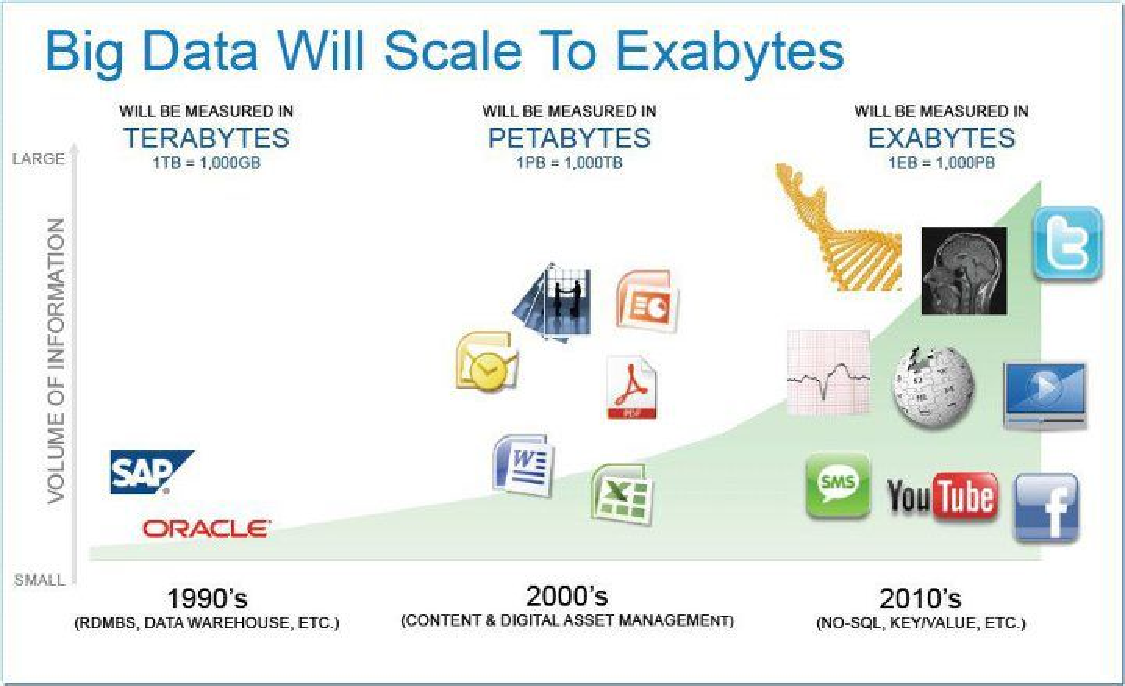
\includegraphics[width=15cm]{template-fig/big_data_exabytes.pdf}
  \caption{S~přibývajícími novými technologiemi se masivně zvyšuje růst dat a~přibývají nové typy \cite{rajeshBigData}.}
  \label{FIG_BigDataExabytes}
\end{figure}

\section{Distribuované databáze}
Distribuovaná databáze se skládá z~většího počtu samostatných databází, které mohou být geograficky rozmístěny na jiných pozicích. Jednotlivé uzly spolu komunikují přes počítačovou síť. Každý uzel je sám o~sobě databázový systém. DSŘBD neboli systém řízení distribuované báze dat (anglicky \texttt{Distributed Database Database Management System}) zajišťuje, že se distribuovaná databáze uživatelům jeví jako jedna jediná databáze. Data jsou fyzicky uložena na různých pozicích. Mohou být spravována rozdílnými SŘBD nezávisle na ostatních pozicích.

\vspace{0.5cm}

\noindent Systém řízení distribuované báze dat je centralizovaný systém s~těmito vlastnostmi 
\cite{distributedDBMS}:

\begin{itemize}
\item Umí vytvářet, získávat, upravovat a~mazat distribuované databáze.

\item Zajišťuje důvěrnost a~integritu databází.

\item Periodicky synchronizuje databázi a~poskytuje mechanismy přístupu tak, aby se databáze uživatelům jevila transparentní.

\item Zajišťuje, že změna dat v~kterémkoliv uzlu se promítne i~v~ostatních uzlech.

\item Je využíván v~aplikacích, kde se předpokládá zpracování velkých objemů dat, ke kterým přistupuje současně mnoho uživatelů.

\item Je navržen pro heterogenní databázové platformy.
\end{itemize}

\begin{figure}[!h]
  \centering
  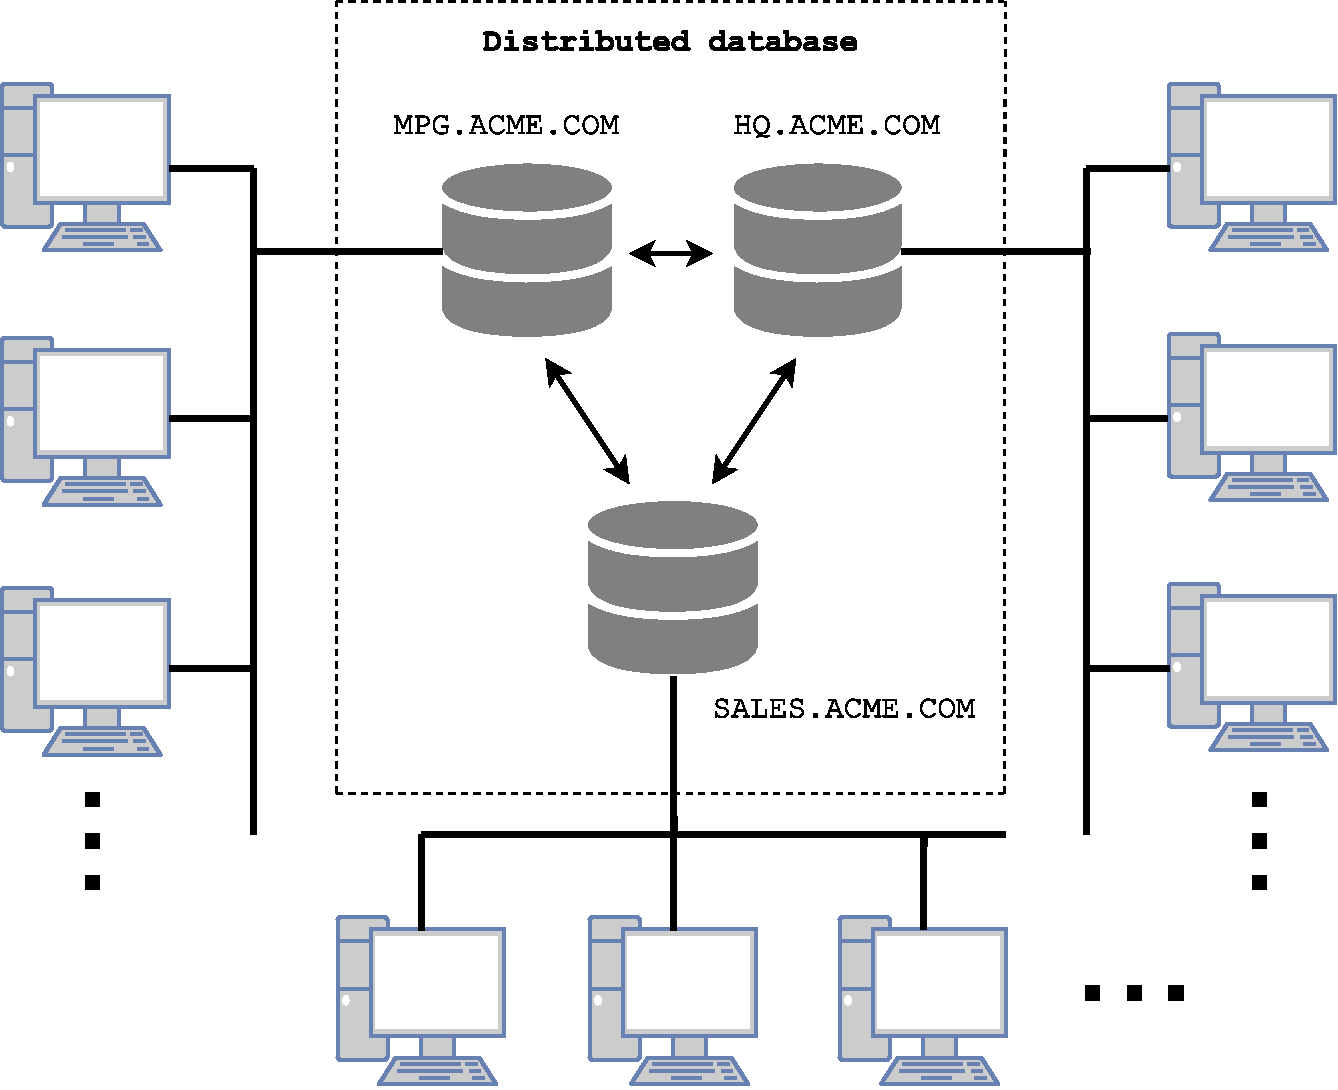
\includegraphics[width=13cm]{template-fig/DistributedDatabase.pdf}
  \caption{Schéma distribuované databáze a~současný přístup více zařízení k~ní \cite{distributedDBMSPic}.}
  \label{FIG_DistrDB}
\end{figure}

\noindent Výhody
\begin{itemize}
\item Rozšiřitelnost -- Pokud je potřeba databázový systém rozšířit do nových míst nebo přidat další uzly, stačí přidat nový(é) počítač(e) a~lokální data v~nové pozici, a~nakonec je připojit k~distribuovanému systému, bez jakéhokoliv přerušení funkcionality. Analogický postup je při odebrání uzlu.

\item Spolehlivost -- Když nějaký z~připojených uzlů selže, nepřestane distribuovaná databáze fungovat, sníží se maximálně výkon.

\item Ochrana (záloha) dat -- Při zničení jednoho uzlu a~smazání dat z~něj, mohou být stejná data zálohována i~na jiných uzlech.

\item Výkonnost -- Pokud jsou data efektivně distribuována, může být uživatelův požadavek uspokojen rychleji. Transakce mohou být také distribuované a~provedeny rychleji. 
\end{itemize}

\noindent Nevýhody
\begin{itemize}
\item CAP teorém -- Pojednává o~tzv. eventuální konzistenci (na rozdíl od absolutní konzistence u~ACID). Definuje, že distribuovaný systém může zajistit maximálně 2 z~těchto 3 vlastností -- konzistence (angl. Consistency), dostupnost (angl. Availability) a~odolnost k~přerušení (angl. Partition tolerance). Je nutné si zvolit mezi konzistencí a~dostupností v~případě výpadku části sítě.

\item Integrita dat -- Data musí být průběžně synchronizována na více uzlech, aby na stejné dotazy nebyly z~různých uzlů vraceny rozdílné odpovědi.

\item Komunikační režie -- I~zdánlivě jednoduchá operace může vyžadovat spoustu zbytečné komunikace.

\item Cena -- DSŘDB vyžaduje drahý a~složitý software ke koordinaci uzlů a~zajištění transparentnosti \cite{distributedDBMS}.

\item Mezi další patří -- složitost, zabezpečení a~řízení souběžného přístupu k~datům.
\end{itemize}

\begin{figure}[!h]
  \centering
  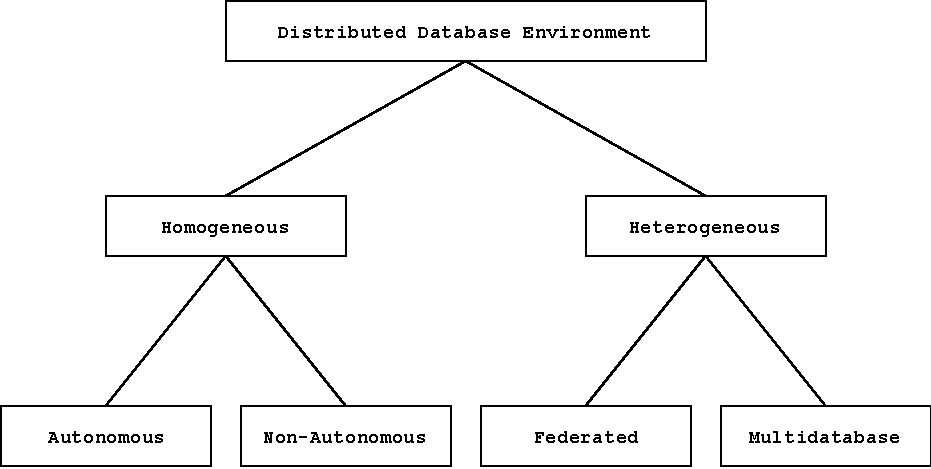
\includegraphics[width=14.2cm]{template-fig/DistributedDatabasesClassification.pdf}
  \caption{Distribuované databáze můžeme podle jejich vlastností dělit \cite{distributedDBMS}.}
  \label{FIG_DivDistrDB}
\end{figure}

\subsection{Rozdělení}
\subsubsection{Homogenní}
Všechny uzly používají identické SŘBD a~operační systémy. Uzly mají informace o~ostatních uzlech a~spolupracují při zpracování uživatelských požadavků. Homogenní distribuovaná databáze se navenek jeví uživateli jako jeden systém. Je jednodušší jej navrhnout a~spravovat.

\vspace{0.5cm}
\noindent Autonomní -- Každá databáze je nezávislá, neexistuje žádný centrální uzel. Databáze jsou spravovány aplikací, a~pro předávání dat používají zasílání zpráv.

\vspace{0.5cm}
\noindent Neautonomní -- Data jsou distribuována napříč homogenními uzly. O~aktualizaci a~správu dat se stará systém řízení distribuované báze dat, který běží na centrálním nebo také master uzlu.

\subsubsection{Heterogenní}
Uzly mohou mít rozdílné operační systémy a~SŘBD, které nejsou kompatibilní. Mohou také využívat rozdílná schémata (relační, objektově orientované, hierarchické, \ldots). Rozdílnost schématu je hlavním problémem při zpracování dotazu a~transakcí. Kvůli tomu je také složité dotazování \cite{wikiDBMS}. Heterogenní distribuované databáze můžeme rozdělit na federované (angl. \texttt{federated}) nebo multidatabázové.

\vspace{0.5cm}
\noindent Architekturami distribuovaných databází jsou centrální architektura, klient-server, peer-to-peer, a~multi-databázová architektura.

\section{Úložiště} \label{storage}
V~této sekci budou popsána strukturovaná a~nestrukturovaná data, jaký je mezi nimi rozdíl a~jaká jsou jejich úložiště.

\subsection{Strukturovaná data}
Strukturovanými daty jsou libovolná data, pro která lze sestavit datový model. Datový model přesně organizuje jednotlivé elementy dat a~specifikuje, jak spolu elementy souvisí, jaké mají vazby, jak budou uloženy, přístup k~nim, a~jak souvisí s~jednotlivými elementy reálného světa \cite{structData}. Typickým úložištěm strukturovaných dat je relační databáze. Pro čtení a~dotazování byl vytvořen dotazovací jazyk SQL.

\subsection{Nestrukturovaná data}
Jak už bylo zmíněno v~sekci \ref{bigDataSection}, Big data patří převážně mezi nestrukturovaná data. Data nemají přesně definovanou strukturu, neexistuje datový model, který by definoval jednotlivé dílčí elementy a~jejich vztahy. Mezi typické zástupce patří: videa, obrázky, audio, webové stránky, text, obsah e-mailové komunikace apod. Mezi vhodná úložiště mohou patřit disková úložiště, NAS (celým názvem \texttt{Network Attached Storage}), HDFS (\texttt{Hadoop Distributed File System}) a~NoSQL databáze.

\subsubsection{NoSQL databáze}
Pod zkratkou se nachází \texttt{non SQL} nebo také \texttt{Not only SQL}. Jedná se o~databázový koncept, ve kterém datové úložiště i~zpracování dat používají jiné prostředky než tabulková schémata tradiční relační databáze \cite{noSqlWiki}. NoSQL databáze jsou navrženy pro distribuovaná ukládání a~dotazování dat, souběžný přístup, a~manipulaci s~obrovským objemem dat. Mezi výhody patří: horizontální i~vertikální škálovatelnost, distribuovaný přístup, flexibilita schématu, dynamičnost. Nevýhodami však mohou být: absence standardizace, omezené schopnosti dotazování, konzistence \cite{noSqlIntro}.

\vspace{0.5cm}
\noindent NoSQL databáze mohou být rozděleny do čtyř kategorií \cite{noSqlOverview}:
\begin{itemize}
    \item Klíč-hodnota (angl. Key-Value databases) -- Jsou nejjednoduššími NoSQL úložišti. Každá položka v~databázi je uložena jako atribut (klíč) společně se svou hodnotou. Hodnota je typu \texttt{blob}, takže pouze aplikace dokáže hodnotu správně interpretovat. Databáze pouze ukládá binární data, kterým nerozumí. Klíč může být složený, např. z~několika částí, které lze použít jako ID do struktury a~nebo ID jejich položek. Klíče mohou být seřazené, což umožňuje efektivní procházení, nebo také organizovány do hierarchií. Zástupci jsou databáze \texttt{Riak} a~\texttt{Redis}.
    
    \item Dokumentové (angl. Document databases) -- Párují každý klíč se složitou datovou strukturou, nazývanou dokument. Představuje v~podstatě princip klíč-hodnota, ale hodnota je strukturovaná. Dokument může obsahovat mnoho rozdílných párů klíč-hodnota, párů klíč-pole, nebo dokonce vnořené dokumenty. Jsou vhodné pro dokumenty formátu XML a~JSON (BSON).
    Databáze dokáže interpretovat strukturovanou hodnotu (dokument), toho lze efektivně využít hlavně při dotazování. Dotazy mohou být i~složitější než přes klíče, např. pomocí \texttt{XPath}. Mezi zástupce patří \texttt{MongoDB} a~\texttt{CouchDB}.
    
    \item Grafové (angl. Graph databases) -- Jsou navrženy pro ukládání entit (uzly) a~jejich vztahů (hrany). Uzly i~hrany mohou mít svoje atributy. Jsou vhodné pro reprezentaci sítí a~jejich topologií, např. sociální či dopravní sítě, topologie počítačových sítí a~další \cite{noSqlPdb}.
    Zástupcem je \texttt{Neo4J}.
    
    \item Sloupcové (angl. Column-oriented databases / Column family stores) -- Data jsou organizována v~tabulkách. Tabulka má řádky jako v~relační databázi, ale u~řádku pak lze definovat sloupce s~hodnotami. Sloupce mohou být pro každý řádek různé (flexibilní schéma), i~různý počet (řídké pole). Sloupcové databáze jsou optimalizovány pro dotazování nad velkými objemy dat. Sloupce mohou být zobecněny na adresáře (anglicky \texttt{supercolumn}), kde potom řádek obsahuje kolekci supersloupců, a~z~nich každý obsahuje kolekci sloupců \cite{noSqlPdb}. Zástupci sloupcových databází jsou například \texttt{Cassandra} a~\texttt{HBase}.
\end{itemize}

\subsection{Srovnání relačních a~NoSQL databází}
Podle výše uvedených vlastností úložišť pro strukturovaná a~nestrukturovaná data můžeme vidět tyto rozdíly:

\begin{multicols}{2}

Relační databáze

\begin{itemize}
    \item Datový model je formalizovaný, databáze umožňuje definovat integritní omezení, kontroly, model reflektuje elementy reálného světa.
    
    \item S~daty lze provádět transformace v~podobě spojení, agregací, řazení apod.
    
    \item Kvůli podpoře transakcí a~ACID vlastností není úplně snadná škálovatelnost.
    
    \item Mají pevné schéma databáze. Vzniklé problémy po úpravách se musí řešit např. migračními skripty.
\end{itemize}

\columnbreak

NoSQL databáze

\begin{itemize}
    \item Jedná se o~nízkoúrovňové úložiště, kde ve většině případů databáze není schopna data interpretovat. Zajištění konzistence je ponecháno aplikaci. 
    
    \item Data lze dostat pouze v~podobě, v~jaké byla uložena.
    
    \item Jsou navrženy pro jednoduchou škálovatelnost.
    
    \item Mají dynamické schéma, které neomezuje definovat libovolnou strukturu a~provádět flexibilní úpravy.
\end{itemize}

\end{multicols}

\chapter{Návrh distribuovaného úložiště} \label{distrRepDesignChapter}
Tato kapitola se zabývá návrhem distribuovaného úložiště rozsáhlých digitálních forenzních dat. Bude popsána komunikace se systémem včetně aplikačního rozhraní, použité technologie, zvolené druhy úložišť a~také zpracování požadavků.

\section{Požadavky na systém}
Nejdůležitějším požadavkem je, aby systém byl distribuovaný, tzn. škálovatelný na více výpočetních uzlech. S~tím souvisí také výběr vhodných technologií.

Systém musí umožnit optimální přístup k~různým datům, jiný přístup bude pro strukturovaná data a~jiný pro nestrukturovaná. Z~forenzních digitálních dat proběhne zaměření převážně na \texttt{PCAP} soubory.

Posledním klíčovým požadavkem je umožnit přidávání podpory pro nové druhy digitálních forenzních dat přímo za běhu systému.

Ze sekce \ref{storage} vyplývá, že je vhodné využít NoSQL distribuovaných databází a~HDFS jako úložiště. Pro komunikaci s~klientem bude sloužit Kafka (společně se ZooKeeper). Všechny tyto technologie jsou distribuované a~ověřené pro použití v~Big data prostředích. Jak jednotlivé technologie fungují bude vysvětleno v~této kapitole.

\section{Aplikační rozhraní}
Aplikační rozhraní umožňuje klientovi komunikovat s~distribuovaným repositářem. Komunikace je založena na asynchronním zasílání zpráv. Systém repositáře nenabízí klientovi přímo žádné metody či funkce, které by klient mohl volat. Ovládání repositáře probíhá pomocí zaslání zprávy obsahující tzv. příkaz. Příkaz specifikuje typ operace a~typ dat. Podle typu příkazu je určeno, jak se daný příkaz zpracuje.

V~následující sekci bude vysvětleno, jak ovládání repositáře probíhá, jak vypadá zpráva, a~bude také uvedeno schéma celé komunikace jako příklad.

\subsection{Komunikace} \label{designCommunication}
Komunikace s~klientem, který chce do distribuovaného repositáře data uložit, nebo naopak z~něj nějaká data získat, probíhá pomocí zaslání zprávy tzv. \texttt{MQ broker}u Kafka. Systém bude pracovat na principu požadavek -- odpověď, ale asynchronním způsobem. Zpráva požadavku obsahuje parametry -- atributy příkazu a~případně řetězec dat.

\vspace{0.5cm}
\noindent Název a~význam parametrů:

\begin{itemize}
    \item \texttt{command} -- Určuje typ příkazu, příklady příkazů mohou být \texttt{STORE\_PCAP} a~\texttt{LOAD\_PCAP}. Příkaz v~sobě ještě zapouzdřuje typ operace, které mohou být \texttt{SAVE} a~\texttt{LOAD}, a~také typ dat jako například \texttt{PCAP}, \texttt{Packet}, \texttt{BINARY}, \texttt{LOG} apod.
    
    \item \texttt{id} -- Povinný parametr, udává unikátní ID zprávy, aby klient potom dokázal identifikovat už zpracované příkazy.
    
    \item \texttt{awaitsResponse} -- Dvoustavová hodnota, jestli klient/odesilatel zprávy očekává od repositáře odpověď. Pokud je tento parametr zadán jako \texttt{True}, je nutné zadat také další parametr \texttt{responseTopic}.
    
    \item \texttt{responseTopic} -- Ve které frontě (angl. topic) je odpověď na straně klienta očekávána.
    
    \item \texttt{errorTopic} -- Na straně distribuovaného úložiště se může vyskytnout chyba, například nedostupnost databáze, chyba při zpracování příkazu a~další. Tento parametr slouží pro zadání fronty, kam se budou zasílat chybová hlášení. Jedná se o~povinný parametr.
    
    \item \texttt{dataSource} -- Zdrojová data k~uložení lze zaslat dvojím způsobem. První z~nich je poslat data v~binární podobě přímo přes systém Kafka společně s~příkazem. Tento způsob lze využít pro data, jejichž velikost není příliš velká, protože se data načítají do paměti RAM. Pro velké objemy dat takový přístup není vhodný. Proto existuje ještě druhý způsob, a~to předat data přes distribuovaný souborový systém HDFS. Parametr dataSource obsahuje název úložiště v~podobě výčtové konstanty \texttt{Kafka} nebo \texttt{HDFS}, cestu k~souboru, pokud se jedná o~HDFS, a~také atribut \texttt{removeAfterUse} pro odstranění souboru po použití. Lze využít i~pro příkazy čtení dat ke způsobu předání výsledku -- přes HDFS nebo Kafku.
    
    \item \texttt{criterias} -- Představuje seznam kritérií pro dotazování. Tento parametr je vhodné vyplnit pouze při zasílání příkazu čtení.
\end{itemize}

\noindent Řetězec dat obsahuje vlastní data, která mají být na straně repositáře zpracována. Typy příkazů, a~v~podstatě typy operací s~typy dat lze libovolně přidávat.

\vspace{0.5cm}
\noindent Zpráva odpovědi nese tyto parametry:
\begin{itemize}
    \item \texttt{id} -- Jedná se o~unikátní ID zkopírované ze zprávy požadavku. Klient po přijetí odpovědi bude vědět, ke kterému požadavku odpověď patří.
    
    \item \texttt{responseTopic} -- Název výstupní fronty, do které je odpověď zaslána.
    
    \item \texttt{responseCode} -- Návratový kód odpovědi symbolizující jak operace dopadla. Analogie s~HTTP návratovými kódy, možnými hodnotami jsou: \texttt{OK(200)}, \texttt{BAD\_REQUEST(400)}, \texttt{UNSUPPORTED\_MEDIA\_TYPE(415)}, \texttt{INTERNAL\_SERVER\_ERROR(500)}.
    
    \item \texttt{status} -- Rezervovaný parametr pro status odpovědi.
    
    \item \texttt{detailMessage} -- Pokud se objeví při zpracování požadavku chyba, může být v~odpovědi odesláno, proč chyba nastala, nebo její přičina.
\end{itemize}

\begin{figure}[!h]
  \centering
  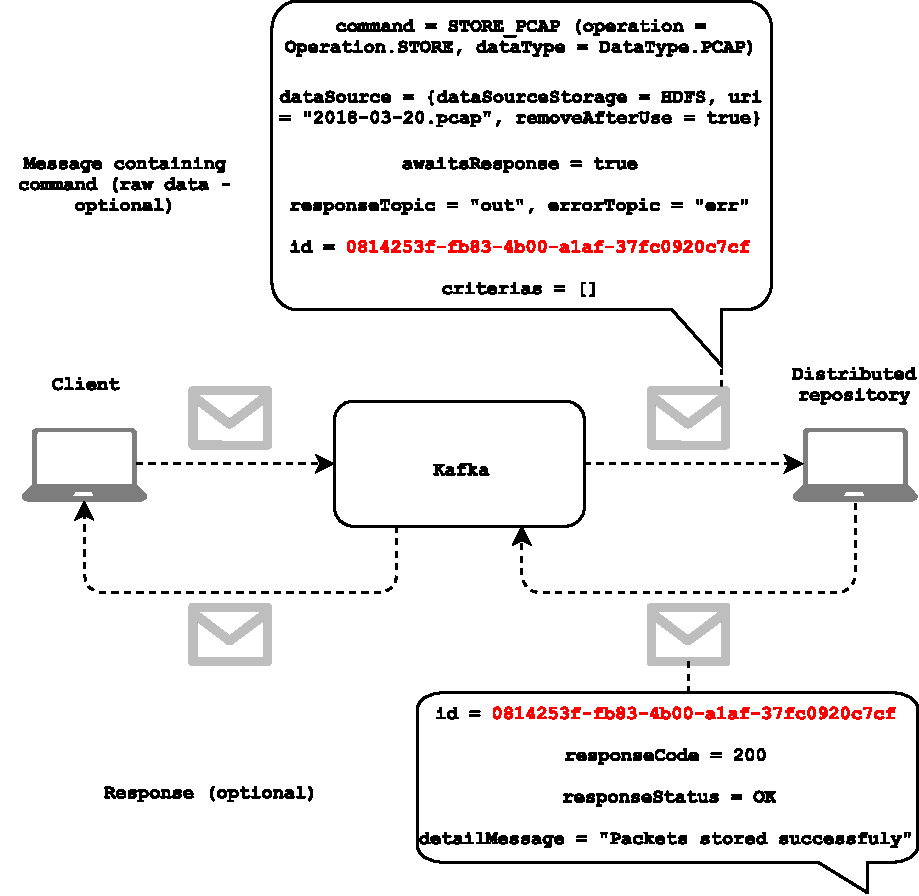
\includegraphics[width=14cm]{template-fig/Kafka_communication.pdf}
  \caption{Demonstrace komunikace -- zaslání zprávy požadavku pro uložení souboru PCAP. Klient zašle příkaz přes Kafku, příkaz je zpracován na straně distr. repositáře, a~případně je odeslána odpověď klientovi. Můžeme si všimnout uvedených ID, jsou stejné -- klient zjistí, ke kterému příkazu odpověď patří.}
  \label{FIG_KafkaCommunication}
\end{figure}

\subsection{Kafka}
Apache Kafka je distribuovaný systém zpráv s~robustními frontami založený na mechanismu \texttt{publish-subscribe} umožňující přenášet vysoké objemy dat. Kafka zprávy jsou perzistentně uloženy na disku a~replikovány v~rámci clusteru kvůli prevenci ztráty dat. Systém Kafka je postaven na synchronizační službě ZooKeeper \cite{kafkaTutorialsPoint}. Výhody jsou:
\begin{itemize}
    \item Spolehlivost -- Kafka je distribuovaný systém, segmentovaný, replikovaný a~odolný proti chybám.
    
    \item Škálovatelnost -- Možnost připojení nových uzlů do clusteru.
    
    \item Odolnost -- Zprávy jsou uloženy na disku.
    
    \item Výkon -- Vysoká propustnost pro obě akce \texttt{publish} a~\texttt{subscribe}. Je zachován stabilní výkon i~při objemu zpráv v~terabajtech.
\end{itemize}

\begin{figure}[!h]
  \centering
  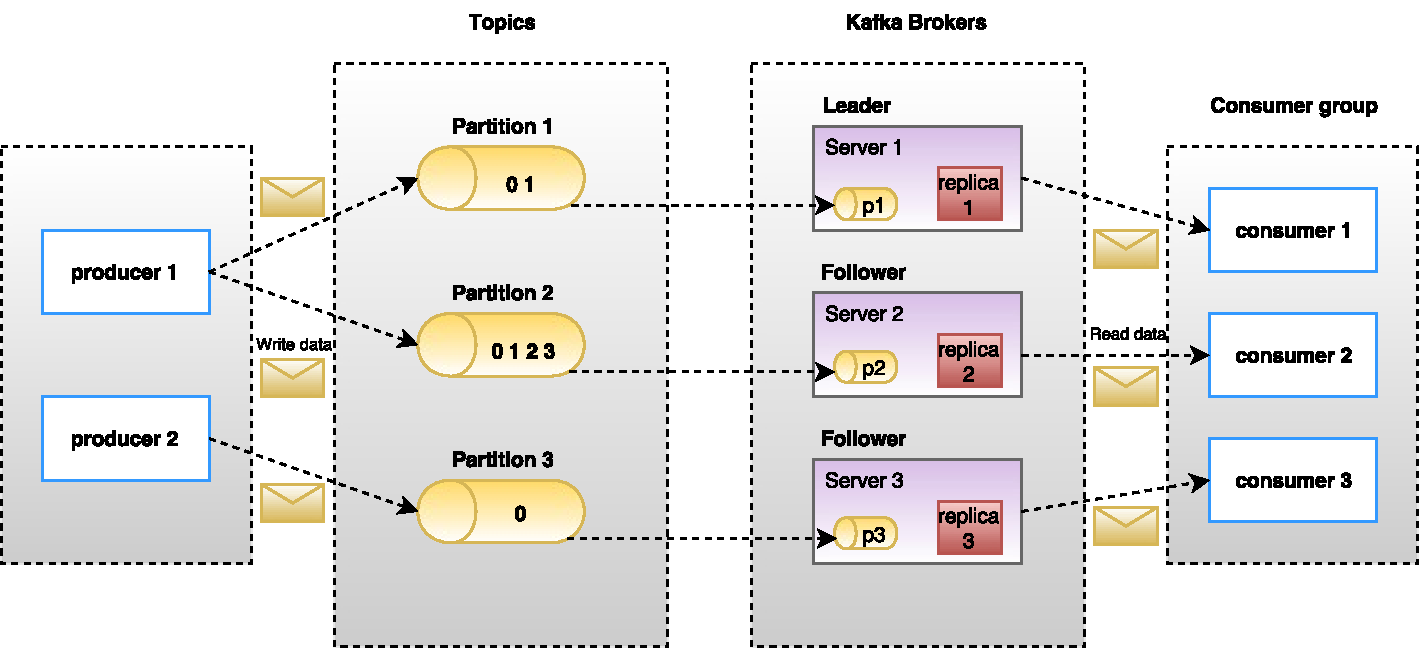
\includegraphics[width=15cm]{template-fig/Kafka_architecture.pdf}
  \caption{Diagram zobrazující klíčové komponenty systému Kafka \cite{kafkaTutorialsPoint}.}
  \label{FIG_KafkaArchitecture}
\end{figure}

\noindent V~diagramu \ref{FIG_KafkaArchitecture} je fronta (angl. \texttt{topic}) konfigurována do tří oddílů (angl. \texttt{partition}). Pokud je faktor replikace fronty nastaven na hodnotu 3, Kafka vytvoří tři identické repliky každého oddílu a~umístí je do clusteru. Každý prostředník (angl. \texttt{broker}) ukládá jeden nebo více těchto oddílů za účelem vyvažování zátěže. Více producentů, respektive konzumentů, může zároveň vydávat (angl. \texttt{publish}), resp. odebírat, (angl. \texttt{subscribe}) zprávy \cite{kafkaTutorialsPoint}.

\vspace{0.5cm}
\noindent Hlavní komponenty systému Kafka z~diagramu \ref{FIG_KafkaArchitecture}:
\begin{itemize}
    \item Fronta -- Jedná se o~proud zpráv patřící k~příslušné kategorii. Data jsou uložena ve frontách. Fronty jsou rozděleny do oddílů.
    
    \item Oddíl -- Fronty mohou mít mnoho oddílů, tak aby zvládaly zpracování libovolného množství dat.

    \item Offset oddílu (angl. \texttt{Partition offset}) -- Každá zpráva v~oddílu má unikátní sekvenci ID nazývanou offset.

    \item Replika oddílu -- Je pouhou zálohou oddílu. Repliky nejsou využívány ke čtení nebo zápisu dat, slouží pouze jako prevence před ztrátou dat.
    
    \item Prostředník -- Jednoduchý systém zodpovědný za správu dat v~oddílech, resp. frontách. Prostředníci slouží k~balancování zátěže.
    
    \item Kafka Cluster -- Pokud existuje víc než jeden prostředník, pak se systém nazývá cluster. Cluster může být rozšířen bez prodlev o~další prostředníky.
    
    \item Producent -- Je odesílatel zprávy do jedné nebo více Kafka front. Producenti posílají data prostředníkům. Pokaždé když producent pošle zprávu prostředníkovi, prostředník přidá zprávu na konec oddílu. Producent nečeká na žádná potvrzení, posílá zprávy tak rychle, jak jen prostředník dokáže přijímat.
    
    \item Konzument -- Čte data od prostředníka(ů). Odebírá z~jedné nebo více front a~konzumuje zprávy vytažením dat od prostředníků.
\end{itemize}

\section{Úložiště}
Tato sekce se zaměřuje na úložiště, kde budou digitální forenzní data uchována. Můžeme je rozdělit na strukturovaná a~nestrukturovaná.

\subsection{Strukturovaná data}
V~souvislosti se systémem repositáře se obecně jedná o~data, která mohou být rozdělena na menší části při zachování možnosti interpretace, a~mohou být efektivně serializována pro uložení. Mezi strukturovaná data můžeme zařadit například soubory formátu PCAP obsahující síťovou komunikaci. Tyto soubory lze rozparsovat na jednotlivé segmenty pakety. Pakety lze potom serializovat na pole bajtů a~uložit do NoSQL databáze. Pro strukturovaná data byla vybrána databáze Cassandra.

\subsubsection{Cassandra}
Jedná se o~zástupce sloupcových NoSQL databází. Výhodami jsou předně: škálovatelnost, odolnost proti chybám, rychlost, distribuovanost, konzistence a~podpora transakcí. Cassandru využívají i~světoznámé společnosti Facebook, Twitter, Cisco, ebay, Twitter, Netflix a~další. Cílem Cassandry je zvládat vysoké objemy dat napříč mnoha uzly. Data jsou pak distribuována na všech uzlech clusteru. Uzly lze libovolně přidávat. Každý uzel je nezávislý a~zároveň propojený s~ostatními. Každý uzel v~clusteru se může podílet na požadavcích čtení či zápisu nezávisle na tom, kde jsou data skutečně uložena. Když uzel selže, požadavky čtení a~zápisu mohou být obslouženy jinými uzly sítě \cite{cassandraTutorialsPoint}.

\subsection{Nestrukturovaná data}
Pro uchování nestrukturovaných dat typu například audio, video, logů, a~obecně binárních dat bude sloužit distribuovaný souborový systém HDFS. Taková data mohou mít velký objem, a~bylo by plýtvání výkonem provádět jejich serializaci nebo rozdělování na části při ukládání do NoSQL databází.

\subsubsection{Hadoop a~HDFS}
Distribuovaný souborový systém HDFS patří pod projekt \texttt{Apache Hadoop}, který je navržen pro ukládání a~zpracování obrovského množství dat v~distribuovaném prostřední napříč mnoha počítači. Počítá se škálovatelností od jednoho serveru po tisíce strojů, kde každý z~nich nabízí lokální úložiště a~výpočetní zdroje \cite{hadoopTutorialsPoint}.

\vspace{0.5cm}
\noindent Platforma Hadoop zahrnuje tyto moduly:

\begin{itemize}
    \item \texttt{Hadoop Common} -- Knihovny a~pomocné nástroje požadované ostatními Hadoop moduly. Poskytují abstrakce souborového a~operačního systému potřebné pro jazyk Java, a~skripty nutné pro spuštění Hadoop-u.
    
    \item \texttt{Hadoop YARN} -- Jedná se o~framework pro plánování distribuovaných úloh a~správu zdrojů.
    
    \item \texttt{HDFS} -- Distribuovaný souborový systém poskytující vysokou propustnost přístupu k~aplikačním datům, škálovatelnost, odolnost proti chybám a~efektivní správu zdrojů.
    
    \item \texttt{Hadoop MapReduce} -- Systém pro paralelní zpracování obrovského množství vstupních dat. Tento modul je pro systém distribuovaného úložiště zbytečný.
\end{itemize}

\noindent Kromě výše uvedených modulů existují i~další pomocné nástroje:  \texttt{Apache Spark}, \texttt{Apache HBase} -- distribuovaná databáze, \texttt{Apache Hive} -- nástroj pro dolování dat nad platformou Hadoop, \texttt{Apache Pig} atd.

\begin{figure}[!h]
  \centering
  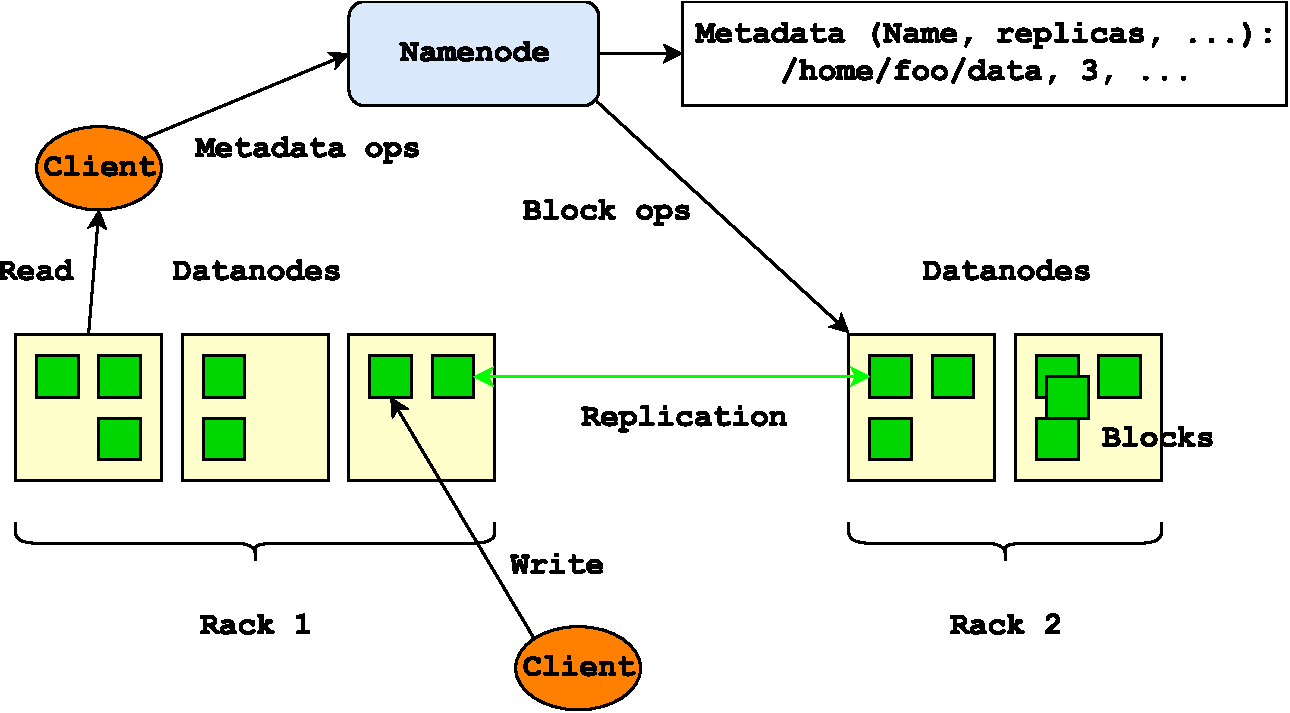
\includegraphics[width=15cm]{template-fig/HDFSArchitecture.pdf}
  \caption{Architektura HDFS \cite{apacheHDFSGuide} -- datové uzly jsou uspořádány do \texttt{rack}-ů, které se nachází v~jedné lokalitě, což zajišťuje rychlejší propojení uzlů. Bloky jsou replikovány mezi odlišné uzly.}
  \label{FIG_HDFSArchitecture}
\end{figure}

\noindent HDFS je virtuální souborový systém vybudovaný nad běžnými souborovými systémy jednotlivých uzlů. Řeší problém nalezení úložiště a~přístupu k~datům, nikoliv fyzické uložení v~uzlu. Byl navržen pro sekvenční přístup k~souborům, nikoliv náhodný \cite{hadoopPdi}.

\noindent HDFS používá architekturu typu \texttt{master/slave}. Master se skládá z~jednoho uzlu nazývaného \texttt{NameNode}, který se stará o~správu metadat a~jmenného prostoru souborového systému. Dále reguluje přístup k~souborům a~provádí operace typu otevření, zavření, přejmenování souborů a~adresářů. Protože je NameNode pouze jeden, měl by být spolehlivý a~výkonný, při jeho výpadku způsobí poruchu systému (jde o~tzv. \texttt{single point of failure}). Uzlů typu slave může být více, jsou nazývány datové uzly (angl. \texttt{DataNodes}), a~ukládají data. Soubor je rozdělen do několika bloků (typicky po 64 nebo 128 MB), a~každý blok souboru je nezávisle replikován v~několika datových uzlech slave. Bloky jsou uloženy v~lokálním souborovém systému na datových uzlech. Datové uzly jsou také zodpovědné za zpracování požadavků čtení a~zápisu od klientů. NameNode se stará o~mapování bloků datovým uzlům, sleduje počet replik jednotlivých bloků. Pokud se nějaká replika ztratí vinou selhání datového uzlu, je vytvořena nová replika bloku \cite{hadoopHortonworks}.

HDFS je implementován v~jazyce Java, na každém stroji s~nainstalovanou Javou může běžet NameNode nebo DataNode software. Typicky při nasazení existuje jeden stroj s~běžícím NameNode, na dalších strojích potom běží datové uzly (lze ovšem najít i~scénáře, kde na jednom stroji běží více datových uzlů). Důležité je, že uživatelská data nikdy neprochází přes NameNode \cite{apacheHDFSGuide}.

\subsection{Metadata} \label{metadata}
V~rámci zpracování příchozí zprávy do repositáře informující o~operaci uložení, by bylo vhodné provést předzpracování dat za účelem vhodnější indexace a~rychlejšího nalezení pro budoucí operace čtení. Jednalo by se tak o~mechanismus podobný například pamětem cache. Uvažme následující scénář pro podrobnější vysvětlení.

Do repositáře bylo v~průběhu několika dnů uloženo mnoho milionů paketů, které obsahovaly síťovou komunikaci mezi několika komunikujícími stranami. Data paketů jsou uložena v~serializované podobě v~NoSQL databázi. Na úrovni databáze nedávají taková data žádný význam, pouze aplikace je dokáže správně interpretovat jako pakety. Po několika dnech by uživatel rád zjistil podrobnější informace o~komunikaci mezi uzly A~a~B. Nezbývalo by mu nic jiného, než všechna data z~NoSQL databáze načíst na aplikační úrovni a~analyzovat paket po paketu, aby zjistil minimálně IP adresy zdroje a~cíle. Takový způsob by byl velmi pomalý a~neefektivní.

Následně uvažme, jak by vypadal postup pro zjištění informací o~komunikaci mezi uzly A~a~B, kdyby byla k~dispozici cache, či paměť metadat. Cache by mohla uchovávat základní informace o~dříve uložených paketech v~jednotně definované struktuře. Mezi tyto informace by patřily -- zdrojová a~cílová IP adresa, zdrojová a~cílová MAC adresa, typ protokolu, časové razítko a~další. Co je však důležité, u~těchto informací by bylo uvedeno ID záznamu z~NoSQL databáze, kde je uchován celý paket. Pro zjištění podrobnějších informací by uživatel mohl načíst pouze ty pakety, které jsou pro něj relevantní.

Předzpracování dat je výhodné před jejich uložením, protože v~kontextu provádění aplikace jsou data interpretovatelná. Výtah základních informací z~nich nezpůsobí propad výkonu. Naopak se výkon zvýší pro případné operace čtení a~hledání.

Výše uvedený princip by se dal zobecnit pro libovolný typ forenzních digitálních dat. Tak by došlo k~vytvoření tzv. registru, který by i~mimo jiné informoval, co je jak a~kde uloženo. Vhodnou strukturou pro uložení těchto metadat může být například formát XML nebo JSON. Z~toho vyplývá použití dokumentové NoSQL databáze jako například MongoDB.

\subsubsection{MongoDB}
MongoDB je multiplatformní, dokumentově orientovaná databáze poskytující vysoký výkon a~dostupnost a~jednoduchou škálovatelnost. Pracuje na principu kolekcí, které nevyžadují schéma. Kolekce je skupina MongoDB dokumentů, a~je ekvivalentem SŘBD tabulek. Dokumenty v~kolekcích mohou mít dynamická schémata a~rozdílné atributy. Dynamické schéma znamená, že dokumenty ve stejné kolekci nemusí mít stejnou strukturu atributů. Počet atributů, obsah a~velikost dokumentu se může mezi dokumenty lišit. Dokument je množina párů klíč-hodnota \cite{mongoDBTutorialsPoint}.

Relační databáze má určité schéma skládající se z~tabulek a~vztahů mezi nimi. Koncept vztahu je v~MongoDB  řešen jinak. Existují dva mechanismy umožňující aplikaci reprezentovat vztahy -- reference a~vnořené dokumenty. Reference uchovávají vztahy mezi daty vložením odkazů (referencí) z~jednoho dokumentu do druhého. Aplikace může díky odkazu přistoupit k~příslušným datům. Vnořené dokumenty zachycují vztahy mezi daty ukládáním příslušných dat přímo do jednoho dokumentu. Namísto atributu dokumentu může být uložen i~jiný dokument. Výhoda tohoto modelu je, že aplikace získá všechna data v~jedné databázové operaci \cite{mongoDBDataModelingIntro}.

Dynamičnost MongoDB je vhodná pro správu metadat, zvlášť když bude do repositáře potřeba přidávat nové druhy dat.

\section{Jádro distribuovaného úložiště}
V~předchozích sekcích byla představena komunikace s~repositářem, jak vypadají příkazy a~jakým způsobem jsou posílána data. Následně byly popsány možnosti ukládání. Tato sekce se zaměřuje na jádro distribuovaného repositáře, převážně na zpracování příkazů a~manipulaci s~databázemi.

Přijetí příkazu zajišťuje konzument zpráv. Konzument se v~krátkých časových intervalech dotazuje na zprávy z~Kafka fronty. Po přijetí zprávy dojde k~přečtení příkazu určeného typem operace a~typem dat společně s~dodatečnými parametry uvedenými v~\ref{designCommunication}. Na základě příkazu dojde k~výběru konkrétní obsluhy (tzv. \texttt{handler}-u), která má za úkol zpracování příkazu. Může se jednat o~uložení dat, o~načtení dat podle zadaných parametrů, přečtení metadat apod. Handler ukrývá všechny potřebné operace, které mají proběhnout při zpracování příkazu. Mimo jiné se jedná i~o~správu metadat zmíněnou v~sekci \ref{metadata}. Při implementaci budou objektu obsluhy nastaveny potřebné závislosti pro řešení databázových operací pro daný typ dat. Každý typ úložiště (souborový systém nebo NoSQL databáze) může mít jiné rozhraní přístupu.

Důležitým požadavkem je, aby úložiště umožňovalo přidávání podpory pro nové druhy forenzních dat za běhu. Tento požadavek je implicitně zajištěn systémem Kafka, který každou přijatou zprávu zapíše na disk a~zpráva tam zůstává, dokud ji konzument úspěšně nezpracuje. V~tom případě lze systém repositáře zastavit, ale Kafka zprávy bude pořád přijímat. Mezitím může proběhnout do-implementování nové funkcionality pro jiný druh forenzních dat, provést kompilaci, nasazení a~spuštění systému. Po spuštění se konzument začne dotazovat Kafky na nové nepřijaté zprávy.

\chapter{Implementace} \label{chapter_impl}

\section{Dekompozice do modulů}
Repositář je komplexní distribuovaný systém, který je postaven na frameworku Spring, sestávající z~několika modulů a~knihoven. V~této sekci je uvedeno, jak byl systém dekomponován do modulů a~jaké knihovny byly zvoleny. Pro správu závislostí a~sestavení aplikace byl zvolen nástroj \texttt{Maven}. Pro přehled byly využity tyto knihovny a~frameworky -- \texttt{Spring Boot}, \texttt{Spring Data}, \texttt{Spring Kafka}, \texttt{Spring Hadoop}, \texttt{Pcap4J}, a~samozřejmě ovladače pro jednotlivé databáze.

Jedná se o~dvě Spring Boot aplikace -- \texttt{DistributedRepository} a~\texttt{ProducerDemo}, které komunikují pomocí komunikačního rozhraní implementovaného v~modulu \texttt{Communication}. Přenos zpráv zajišťuje projekt Spring Kafka. Aplikace DistributedRepository má přístup k~oběma databázím Cassandra a~MongoDB díky modulu \texttt{Persistence} obsahujícím mimo jiné projekt Spring Data, a~také k~HDFS pomocí projektu Spring Hadoop. K~HDFS má přístup i~klientská aplikace ProducerDemo.

\begin{figure}[!h]
  \centering
  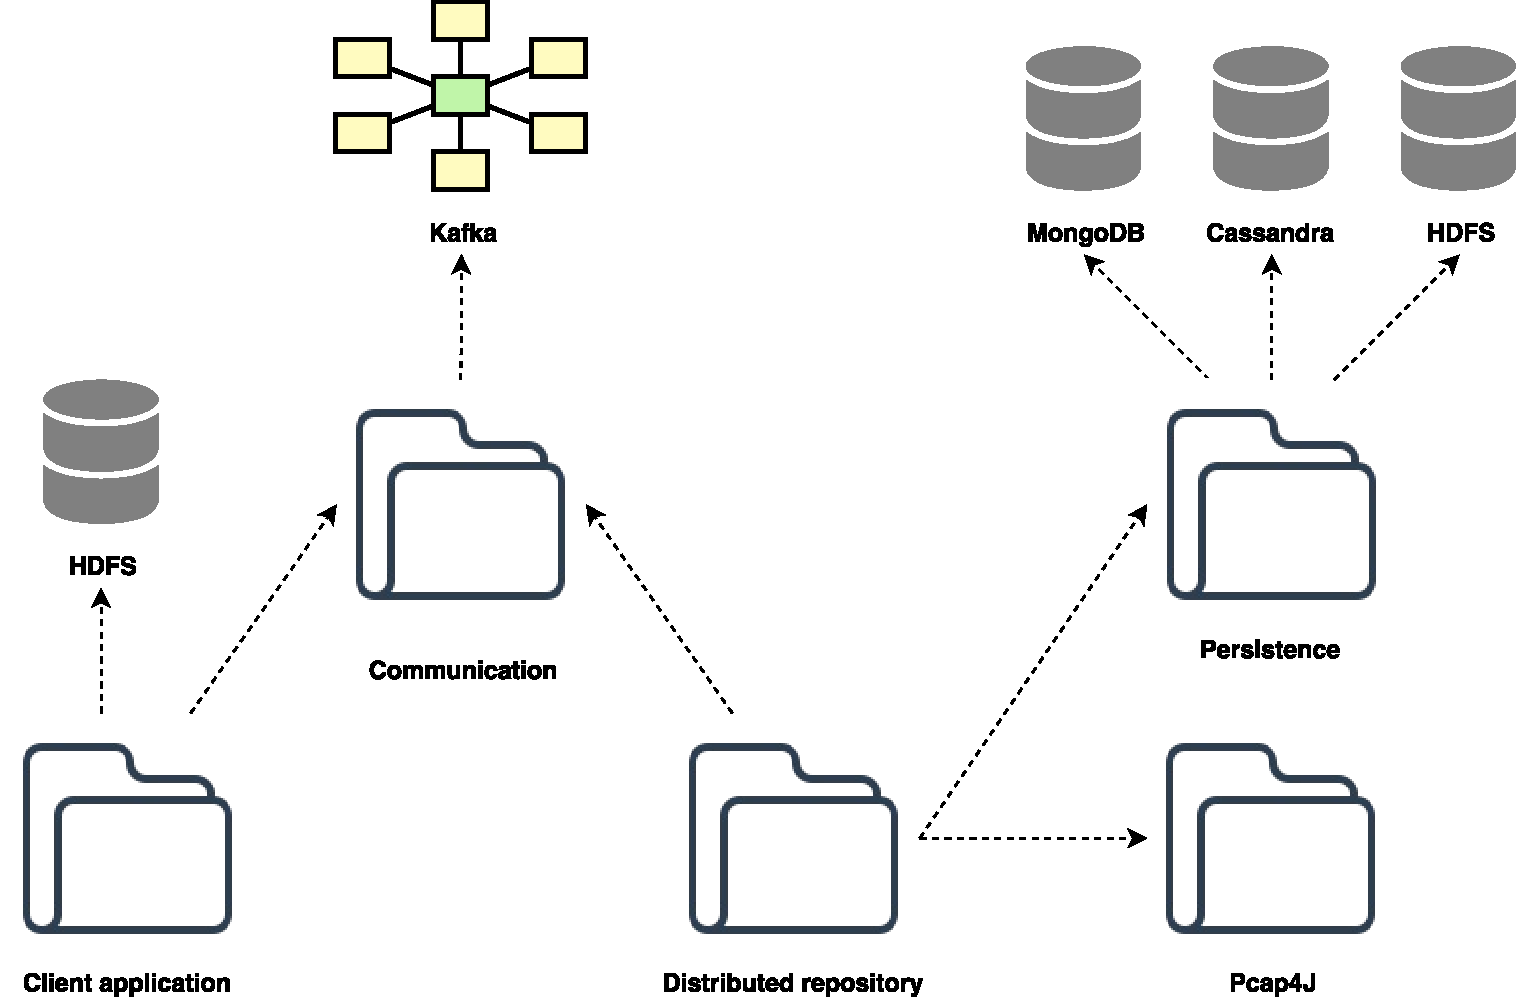
\includegraphics[width=12.3cm]{template-fig/Architecture.pdf}
  \caption{Schéma klíčových modulů a~závislostí systému.}
  \label{FIG_Architecture}
\end{figure}

\subsection{Pcap4J} \label{pcap4j}
Jedná se o~knihovnu pro jazyk Java pro zachytávání, konstruování a~odesílání paketů. Knihovna je stále ve vývoji. Pcap4J pracuje nad nativní knihovnou (\texttt{libpcap}, \texttt{WinPcap}, nebo \texttt{Npcap} v~závislosti na operačním systému) přes JNA (\texttt{Java Native Access})
\footnote{https://github.com/java-native-access/jna}
a~poskytuje aplikační rozhraní pro jazyk Java. Mimo výše uvedené činnosti dokáže pracovat s~PCAP soubory, vytvářet a~parsovat je na jednotlivé pakety. Každý paket implementuje rozhraní \texttt{Packet}. Toto rozhraní nabízí mimo jiné dvě klíčové metody \texttt{contains} a~\texttt{get}. Metoda \texttt{contains} slouží ke kontrole, jestli je paket konkrétního typu, který chceme získat. Metoda má jako parametr třídu, které je paket typem, hlavička metody potom vypadá:

\begin{lstlisting}[language=Java]
    boolean contains(Class<T> clazz)
\end{lstlisting}

\noindent Ke konkrétnímu typu paketu, např. IP paketu, se přistupuje pomocí reflexe voláním metody:

\begin{lstlisting}[language=Java]
    T get(Class<T> clazz)
\end{lstlisting}

\noindent Tedy například:

\begin{lstlisting}[language=Java]
    IPv4Packet ipv4Packet = ethernetPacket.get(IPv4Packet.class);
\end{lstlisting}

\noindent Návratová hodnota metody \texttt{get} je objekt třídy uvedené v~parametru. Před voláním \texttt{get} je vhodné zkontrolovat typ pomocí metody \texttt{contains}. Z~konkrétního paketu už lze získávat potřebné informace, v~případě IP paketu údaje z~hlavičky jako zdrojová a~cílová IP adresa, verze protokolu apod. Analogicky lze postupovat i~v~případě ostatním typů paketů, Z~TCP paketu lze získat údaje o~portech, sekvenční čísla, kontrolní součet a~další.

Knihovna reflektuje zapouzdření, které spočívá ve vložení protokolové datové jednotky (anglicky \texttt{Protocol Data Unit}) vyšší vrstvy do protokolové jednotky nižší vrstvy. Takže ethernetový paket může být současně i~IP paketem a~podobně.

\begin{figure}[!h]
  \centering
  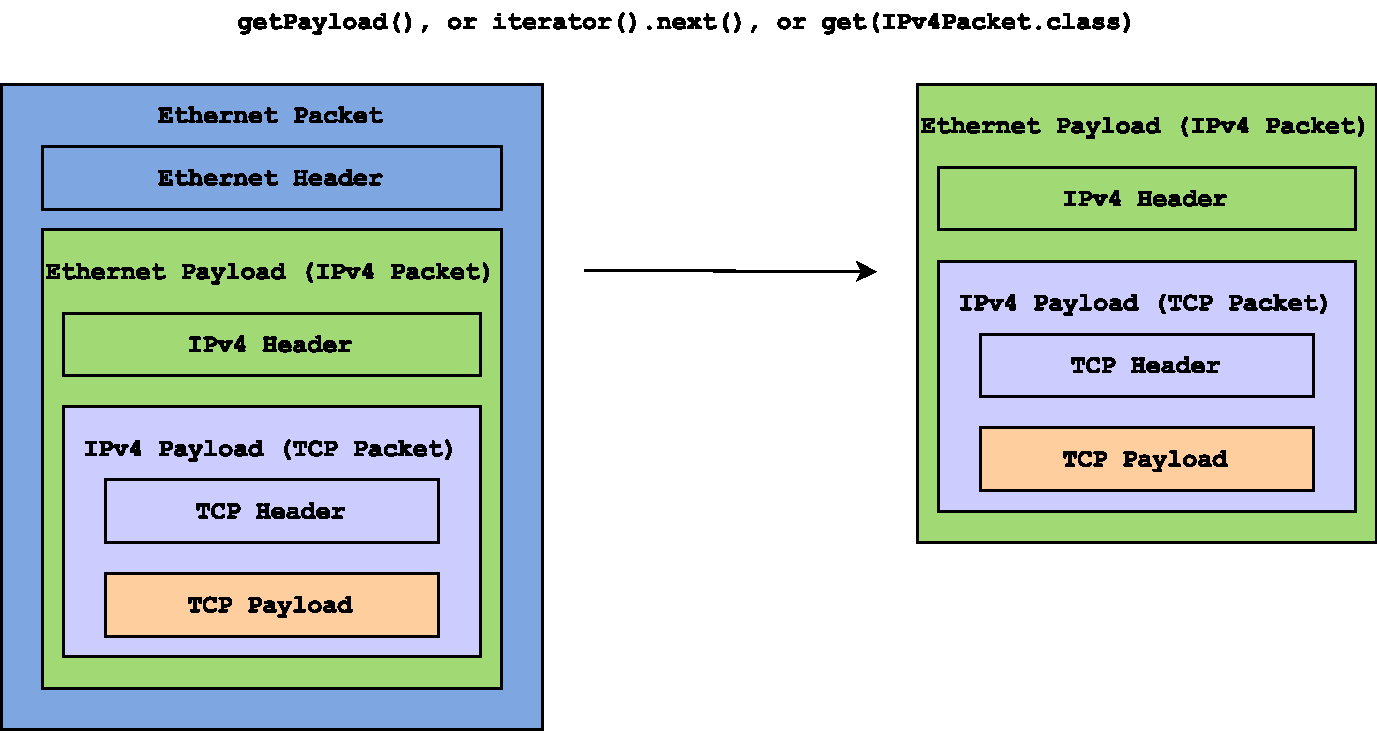
\includegraphics[width=15cm]{template-fig/Pcap4JExample.pdf}
  \caption{Schéma znázorňující výše uvedený příklad pro manipulaci s~pakety \cite{gitPcap4J}.}
  \label{FIG_Pcap4JExample}
\end{figure}

\subsection{Spring, Spring Boot a~Spring projekty}
Spring je velmi populární framework pro jazyk Java umožňující vytvářet webové a~enterprise aplikace. Věnuje se mnoha obecným principům a~problémům jako jsou například \texttt{dependency injection}, konfigurace, aspektově orientované programování, ORM, validace, bezpečnost, testování, integrace s~jinými frameworky atd. V~současné době pod něj spadají desítky projektů, každý zaměřený na jiný aspekt \footnote{https://spring.io/docs/reference}.

Spring poskytuje tři způsoby konfigurace -- pomocí XML, anotací a~konfigurace přímo v~Java. S~rozšiřující se funkcionalitou se zvyšuje komplexita a~i~konfigurace se stává obtížná a~náchylná k~chybám. Z~důvodu lepšího způsobu konfigurace byl vyvinut Spring Boot. Spring Boot přichází s~principem auto-konfigurace, ponechává však možnost předefinovat výchozí nastavení. Klíčovými vlastnostmi jsou \cite{whySpringBoot}:

\begin{itemize}
    \item Jednoduchá správa závislostí -- Pokud chceme použít Spring Boot k~běhu aplikace, je potřeba importovat \texttt{spring-boot-starter-parent} jako modulovou závislost. Existují další \texttt{Spring Boot Starter} závislosti, které se hodí pro určitý typ nebo aspekt vyvíjené aplikace. Existují např. \texttt{Test Starter}, \texttt{Web Starter}, \texttt{Security Starter}, \texttt{Data JPA Starter}, \texttt{AOP Starter} atd. Pokud chceme vyvíjet např. webovou aplikaci, Web Starter poskytne všechny potřebné závislosti zahrnující MVC modul, validační API, prostředky k~serializaci dat atp. Webová aplikace typicky potřebuje pracovat s~databází -- Data JPA Starter poskytne všechny potřebné závislosti zahrnující transakční API, \texttt{Hibernate} knihovny, ORM implementaci atd.
    
    \item Auto-konfigurace -- Nejenže Starter Web poskytne potřebné závislosti, ale proběhne konfigurace běžně používaných objektů tříd \texttt{ResourceHandlers}, \texttt{MessageSource} atd. výchozími hodnotami. Analogicky proběhne konfigurace objektů nutných k~používání JPA -- \texttt{DataSource}, \texttt{TransactionManager} a~\texttt{EntityManagerFactory}. Uživatel tyto objekty sám nevytváří, o~jejich vytvoření se postará Spring Boot na základě poskytnutých údajů v~konfiguračním souboru \texttt{application.properties} (příklad konfigurace aplikace uveden v~\ref{configuration}). Spring Boot tedy podle zdrojů uvedených v~\texttt{classpath} provádí konfiguraci celé aplikace.
    
    \item Podpora zabudovaného kontejneru -- Pokud vyvíjíme webovou aplikaci, která bude běžet v~nějakém kontejneru typu \texttt{Tomcat}, není potřeba provádět žádná nasazení do externího kontejneru. Kontejner je při kompilaci automaticky stažen spolu s~ostatními závislostmi a~je zabudovaný, takže aplikaci stačí pouze spustit a~Spring Boot se postará o~nasazení do zabudovaného kontejneru. Samozřejmě lze zvolit i~jiný typ kontejneru, např. \texttt{Jetty} apod.
\end{itemize}

\noindent Spring Boot umožňuje vytvářet tzv. \texttt{beans} přímo v~Java kódu, bez použití XML konfiguračních souborů. Každou bean lze vytvořit pomocí anotace \texttt{@Bean}, např.

\begin{lstlisting}[language=Java,frame=tb,basicstyle={\small\ttfamily}]
@Configuration
public class ParserBeans {
    @Bean
    public PcapParser<PcapPacket> pcapParser() {
        return new ParserImpl();
    }
}
\end{lstlisting}

\noindent Použití vytvořené bean je velmi jednoduché pomocí anotace \texttt{@Autowired}:

\begin{lstlisting}[language=Java,frame=tb,basicstyle={\small\ttfamily}]
@Autowired
private PcapParser<PcapPacket> pcapParser;
\end{lstlisting}

\noindent Uživatel tedy definoval bean v~konfigurační třídě označené anotací \texttt{@Configuration}, a~tato instance je pak dodána principem dependency injection.

\subsubsection{Spring Kafka} \label{springKafka}
Projekt Spring Kafka aplikuje klíčové koncepty Springu pro vývoj systémů založených na platformě Kafka. Poskytuje šablonu jako vysokoúrovňovou abstrakci pro zasílání zpráv \cite{springKafka}. Velkým přínosem je výše zmíněná auto-konfigurace ze zadaných parametrů, která umožňuje okamžité použití komponent bez vytváření instancí uživatelem.

Mezi nejdůležitější třídy patří \texttt{KafkaTemplate}, která zapouzdřuje mnoho metod pro odeslání zpráv do Kafka front. Podporuje asynchronní i~synchronní odesílání. Použití této šablony lze vidět ve třídě \texttt{ResponseProducer} z~diagramu tříd \ref{FIG_CommunicationClassDiagram}.

Zprávy mohou být přijímány pomocí zvoleného kontejneru \texttt{MessageListenerContainer}, který poskytuje implementaci tzv. \texttt{Message Listener} nebo je označen pomocí anotace \texttt{@KafkaListener}. Existují 2 implementace kontejneru -- \texttt{KafkaMessageListenerContainer} (aktuálně použitá implementace v~systému repositáře), kde jsou přijímány všechny zprávy ze všech front a~oddílů v~jednom vláknu; a~\texttt{ConcurrentMessageListenerContainer}, který deleguje zpracování 1 nebo více kontejnerům, což poskytuje vícevláknový odběr zpráv a~tudíž i~vícevláknové zpracování \cite{springKafka}, více v~\footnote{https://docs.spring.io/spring-kafka/docs/2.1.6.BUILD-SNAPSHOT/reference/html/\_reference.html}. Lze také nastavit různé filtry a~vzorce pro přijímané zprávy, a~rozdělit tak příjem zpráv podle jejich struktury jiným objektům.

\subsubsection{Spring Hadoop}
Další z~projektů, které patří pod Spring, je Spring Hadoop, zjednodušující použití Hadoop API pro Javu. Přináší zase výše zmíněný jednotný konfigurační model usnadňující vývoj systémů postavených na platformě Hadoop, využívající HDFS, paradigma MapReduce, Hive a~Pig. Poskytuje také integraci s~jinými projekty ze Spring ekosystému jako například \texttt{Spring Integration} a~\texttt{Spring Batch}. Podporuje tvorbu Hadoop aplikací, které jsou konfigurovány principem dependency injection a~spuštěny jako standardní Java aplikace nebo pomocí nástrojů Hadoop pro příkazovou řádku.
Velmi jednoduše lze integrovat se Spring Boot pro zjednodušení připojení k~HDFS za účelem manipulace s~daty \cite{springHadoop}. Jedná se o~komplexní systém obsahující obrovské množství dalších nástrojů, podsystémů a~nastavení, které ovšem překračují použití v~distribuovaném úložišti, více lze nalézt na referenčních webových stránkách projektu Spring Hadoop \footnote{https://docs.spring.io/spring-hadoop/docs/2.5.1.BUILD-SNAPSHOT/reference/html/}.

Pro účely distribuovaného repositáře byla využita převážně možnost propojení s~HDFS. Přistupovat k~HDFS lze obecně několika způsoby -- použít Java API \footnote{https://hadoop.apache.org/docs/r2.7.3/api/org/apache/hadoop/fs/FileSystem.html} (nutno stále kontrolovat výjimky a~ošetřovat chybové stavy), nebo souborový systém ovládat pomocí příkazové řádky nástrojem \texttt{hadoop} \footnote{https://hadoop.apache.org/docs/r2.7.3/hadoop-project-dist/hadoop-common/FileSystemShell.html} mimo Java aplikaci. Oba způsoby nejsou uživatelsky přívětivé. Spring Hadoop propojuje tyto dva způsoby skrze intuitivní jednoduché Java API \cite{springHadoopReference}.

HDFS nabízí tři API:
\begin{table}[h!]
    \centering
    \begin{tabular}{| l | l | l | l | l |}
    \hline
    Soubor. systém   &   Metoda   &   Schéma/Prefix &  Zápis/Čtení &   Verze \\ \hline
    HDFS & RPC & \texttt{hdfs://} & Zápis i~čtení & Pouze stejná verze \\ \hline
    HFTP & HTTP & \texttt{hftp://} & Pouze čtení & Nezávislé na verzi \\ \hline
    WebHDFS & HTTP (REST) & \texttt{webhdfs://} & Zápis i~čtení & Nezávislé na verzi \\ \hline
    \end{tabular}\par
    \bigskip
    \caption{Druhy API, které HDFS poskytuje, převzato z~referenční dokumentace \cite{springHadoopReference}.}
    \label{HDFSApi}
\end{table}

\noindent Pro účely distribuovaného úložiště bylo zvoleno první API, tzv. HDFS, založené na RPC volání -- tento způsob vyžaduje, aby klient i~Hadoop cluster běželi na stejné verzi (rozdílné verze způsobí problémy v~serializaci). Další alternativou by bylo API WebHDFS, které ovšem vyžaduje další konfiguraci, a~přenos pomocí HTTP přináší režii navíc ve formě zpomalení ukládání a~čtení dat.
API HFTP v~tomto případě využít nelze, protože podporuje pouze čtení.

Praktickým nástrojem poskytovaným distribucí Hadoop je klient příkazové řádky, přes kterého lze spouštět příkazy podobné těm linuxovým přímo nad HDFS -- existenci, mazaní, kopírování, přesouvání souborů, nebo nastavení přístupových práv. Tento nástroj je dostupný pouze přes příkazovou řádku, což stěžuje použití přímo z~Java aplikace. Spring Hadoop poskytuje plně zabudovanou funkcionalitu výše zmíněného nástroje uvnitř třídy \texttt{FsShell}, která zrcadlí většinu příkazů dostupných z~příkazové řádky (metody typu \texttt{chmod}, \texttt{cp}, \texttt{copyFromLocal}, \texttt{get}, \texttt{ls}, \texttt{mkdir}, \texttt{put}, \texttt{rm}, atd) \cite{springHadoopReference}. Pomocí této třídy jsou prováděny veškeré operace s~HDFS.

\section{Úložiště}
Jak už bylo uvedeno v~kapitole \ref{distrRepDesignChapter}, úložiště je tvořeno NoSQL databázemi Cassandra a~MongoDB, a~distribuovaným souborovým systémem HDFS. Zatímco předešlá kapitola jen nastínila vlastnosti těchto úložišť, zde budou vysvětleny technické detaily a~práce s~nimi.

\subsection{Cassandra} \label{cassandra}
Schéma databáze Cassandra je aktuálně velmi jednoduché. Nejzevnější úroveň tvoří tzv. \texttt{Keyspace} představující kontejner tabulek. Keyspace svými atributy udává replikační faktor (angl. \texttt{replication factor}), strategii umísťování replik (angl. \texttt{replica placement strategy}), a~třídy sloupců (angl. \texttt{column families}). Aktuální nastavení keyspace vypadá následovně:

\vspace{0.5cm}
\texttt{CREATE KEYSPACE structured\_data WITH replication = }

\texttt{\string{ 'class':'SimpleStrategy', 'replication\_factor':1 \string} }

\vspace{0.5cm}
\noindent Je použita strategie \texttt{SimpleStrategy}, vhodná pouze pro jedno sdružení počítačových uzlů (\texttt{rack}). Není optimální pro současné použití mnoha datovými centry, k~tomu slouží strategie \texttt{NetworkTopologyStrategy}. Replikační faktor vyjadřuje počet strojů v~clusteru, které obdrží stejnou kopii dat. Zde nastaveno na hodnotu 1.

Schéma tabulky pro ukládání paketů je taktéž velmi jednoduché. Tabulka obsahuje pouze primární klíč ID a~hodnotu paketu v~binární podobě. Struktura tabulky:

\vspace{0.5cm}
\texttt{packet (
	id timeuuid PRIMARY KEY,
	packet blob
)}

\subsubsection{Asynchronní dotazy}
Distribuovaný repositář komunikuje s~databází asynchronně z~důvodu co největší propustnosti a~rychlosti. Asynchronní komunikace je umožněna díky třídám a~metodám ovladače pro jazyk Java od společnosti DataStax, který je stále ve vývoji \footnote{https://github.com/datastax/java-driver}. Tento ovladač používá asynchronní architekturu. Takový způsob komunikace dovoluje klientské aplikaci ukládat data a~provádět nad nimi dotazy neblokujícím způsobem, díky tzv. \texttt{Future} instancím \cite{asyncQueriesCassandra}.

\begin{figure}[!h]
  \centering
  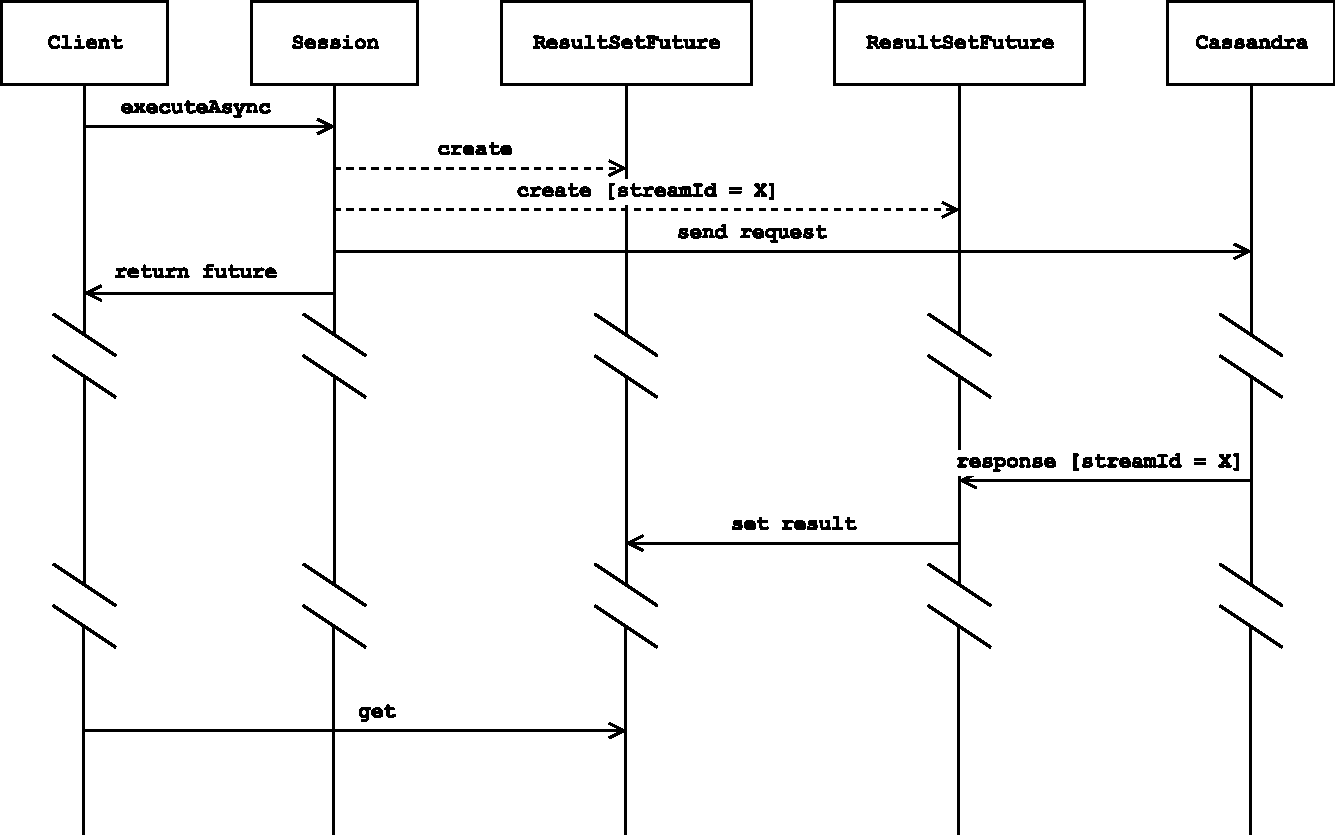
\includegraphics[width=15cm]{template-fig/CassandraAsyncQueries.pdf}
  \caption{Sekvenční diagram znázorňující jednotlivá volání metod při vykonávání asynchronního dotazu do databáze Cassandra \cite{asyncQueriesCassandra}.}
  \label{FIG_CassandraAsyncQueries}
\end{figure}

\noindent Kromě zaslání dotazu do databáze, ovladač registruje interní obsluhu v~podobě objektu \texttt{ResponseHandler}, který zpracuje odpověď dotazu, až bude k~dispozici. Po zaregistrování obsluhy je předáno řízení vykonávání volajícímu programu společně s~objektem třídy \texttt{ResultSetFuture}, pomocí kterého klient dokáže získat výsledek dotazu a~dále s~ním pracovat.
Až databáze dotaz dokončí a~vrátí odpověď, ovladač avizuje ResponseHandler (obecně může být zaregistrováno mnoho takových obsluh pro různé dotazy, párování je provedeno pomocí unikátního ID \texttt{streamId}, které bylo zasláno s~dotazem). Obsluha třídy ResponseHandler dokončí volání upozorněním objektu třídy ResultSetFuture.
Klientský kód získá výsledek dotazu provedením metody \texttt{get} nad objektem ResultSetFuture. Volání této metody je blokující, pokud ještě nebyl nastaven výsledek objektu ResultSetFuture \cite{asyncQueriesCassandra}.

Čekat na výsledek blokujícím způsobem není efektivní, proto existuje i~způsob bez blokování. V~takovém případě musí klient k~objektu ResultSetFuture zaregistrovat svůj tzv. \texttt{callback}, který bude vykonán, až bude výsledek k~dispozici.
Lze zvolit i~jiné vlákno pro jeho vykonání, aby aktuálně běžící kód nemusel být pozastaven. To lze například pomocí knihovny \texttt{Guava} od Google a~jejich tříd \texttt{Futures} a~\texttt{FutureCallback}.

\noindent Ovladač od DataStax je obecně celý asynchronní, uvnitř jeho synchronních metod je zavolána asynchronní verze, a~pak okamžitě blokující metoda get. Ovladač umožňuje paralelně provádět pouze omezený počet dotazů. Tento počet je udán vnitřními parametry \texttt{Cluster} objektu (více detailních informací lze nalézt na referenčních www stránkách ovladače v~sekci \texttt{Connection pooling} \footnote{https://docs.datastax.com/en/developer/java-driver/2.1/manual/pooling/}):

\begin{itemize}
    \item \texttt{maxRequestsPerConnection} -- Udává maximální počet požadavků na jedno připojení.
    
    \item \texttt{maxConnectionsPerHost} -- Udává maximální počet připojení na uzel.
\end{itemize}

\noindent Počet paralelních připojení do databáze Cassandra je v~systému limitován semaforem. Jinak by vždy při vyčerpání dostupných připojení docházelo k~selhání ve formě výjimky \texttt{NoHostAvailableException}. Při každém dotazu do databáze, čtení nebo zápis, tedy dojde k~uzamčení semaforu, při dokončení operace (či při chybě) zase k~odemknutí semaforu. Semafor byl nastaven na počet přístupů daných výrazem:

\vspace{0.5cm}
\texttt{maxConnectionsPerHost * maxRequestsPerConnection}

\vspace{0.5cm}
\noindent Tímto přístupem je tedy maximálně využito systémových prostředků a~docíleno zrychlení provádění dotazů.

\subsection{MongoDB} \label{mongoDB}

\begin{figure}[!h]
  \centering
  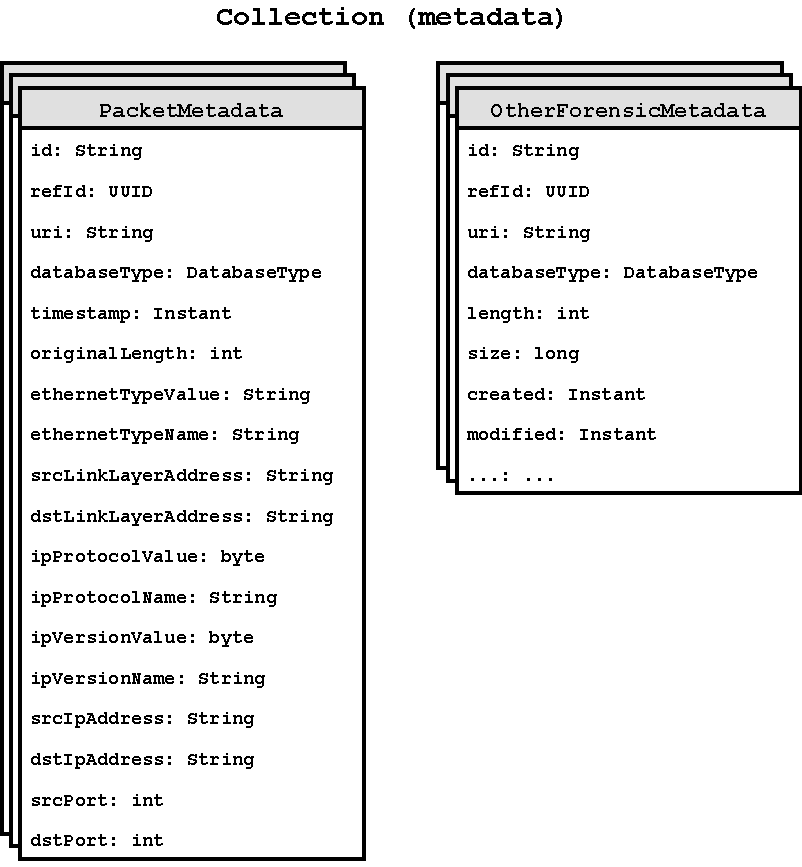
\includegraphics[width=13cm]{template-fig/MetadataSchema.pdf}
  \caption{Schéma databáze pro metadata, obsahuje zatím pouze metadata pro pakety sdružované v~kolekci dokumentů typu PacketMetadata. Kolekce dokumentů typu \texttt{OtherForensicMetadata} je zde uvedena jako příklad pro rozšíření do budoucna.}
  \label{FIG_MetadataSchema}
\end{figure}

MongoDB slouží k~uchování registru metadat. Důvody k~zavedení podsystému metadat jsou uvedeny v~\ref{metadata}. Druh metadat pro nějaký typ forenzních dat lze reprezentovat jako dokument ve formátu JSON. Dokumenty stejného typu jsou pak ukládány do kolekce. Pro každý typ ukládaných forenzních dat existuje takový dokument. Při ukládání dat do Cassandry nebo HDFS je dokument metadat sestaven a~vyplněn klíčovými atributy, podle kterých bude možné později vyhledávat.

\vspace{0.5cm}
\noindent Pro pakety byl zvolen dokument typu \texttt{PacketMetadata} s~těmito atributy:

\begin{itemize}
    \item \texttt{id} -- Unikátní ID v~rámci MongoDB.
    
    \item \texttt{refId} -- Unikátní ID pro záznamy v~databázi Cassandra.
    
    \item \texttt{uri} -- Pokud jsou korespondující forenzní data uložena v~HDFS, je vyplněn tento atribut cestou k~datům v~HDFS.
    
    \item \texttt{databaseType} -- Určuje typ úložiště, povolenými hodnotami jsou \texttt{Cassandra} a~\texttt{HDFS}.
    
    \item \texttt{timestamp} -- Časové razítko paketu.
    
    \item \texttt{originalLength} -- Délka paketu v~bajtech.
    
    \item \texttt{ethernetTypeValue} -- Hodnota z~ethernetové hlavičky paketu, která udává typ protokolu v~hexadecimálním formátu, např. 0x0800 pro IPv4, 0x86dd pro IPv6 atd.
    
    \item \texttt{ethernetTypeName} -- Hodnota z~ethernetové hlavičky paketu, která udává typ protokolu v~řetězcovém formátu, např. IPv4, IPv6, ARP atd.
    
    \item \texttt{srcLinkLayerAddress} -- Zdrojová fyzická adresa ve formátu \texttt{xx:xx:xx:xx:xx:xx}.
    
    \item \texttt{dstLinkLayerAddress} -- Cílová fyzická adresa ve formátu \texttt{xx:xx:xx:xx:xx:xx}.
    
    \item \texttt{ipProtocolValue} -- Hodnota z~IP hlavičky paketu, která udává typ transportního protokolu v~celočíselném formátu, např. 4 pro ICMPv4, 6 pro TCP, 17 pro UDP atd.
    
    \item \texttt{ipProtocolName} -- Hodnota z~IP hlavičky paketu, která udává typ transportního protokolu v~řetězcovém formátu, např ICMPv4, IGMP, TCP, IGP atd.
    
    \item \texttt{ipVersionValue} -- Hodnota z~IP hlavičky paketu udávající číslo verze IP protokolu, 4 pro IPv4, 5 pro ST, 6 pro IPv6 apod.
    
    \item \texttt{ipVersionName} -- Hodnota z~IP hlavičky paketu udávající verzi IP protokolu v~řetězcovém formátu, např. IPv4, ST, IPv6 atd.
    
    \item \texttt{srcIpAddress} -- Zdrojová IP adresa v~řetězcovém formátu, lze tedy uchovat IPv4 i~IPv6 adresu. IPv6 adresa může mít více řetězcových interpretací, např. řetězce \texttt{ff02:0:0:0:0:0:0:c} a~\texttt{ff02::c} vyjadřují tu samou IPv6 adresu. IP adresy jsou získány z~paketu pomocí knihovny Pcap4J \ref{pcap4j}, která IP adresy vrací jako Java objekty typu \texttt{InetAddress}. Tyto objekty nelze serializovat do databáze, proto jsou ukládány jen řetězcové hodnoty. Nicméně třída InetAddress nabízí statickou metodu \texttt{InetAddress 	getByName(String host)}, kterou lze IP adresy normalizovat na stejný řetězcový tvar. Obě následující volání vrátí stejný řetězec:
    
    \indent \texttt{InetAddress.getByName("ff02:0:0:0:0:0:0:c").getHostAddress()}
    
    \indent \texttt{InetAddress.getByName("ff02::c").getHostAddress()}
    
    \item \texttt{dstIpAddress} -- Cílová IP adresa ve stejném formátu jako zdrojová.
    
    \item \texttt{srcPort} -- Zdrojový port.
    
    \item \texttt{dstPort} -- Cílový port.
\end{itemize}

\noindent První čtyři atributy jsou společné pro všechny druhy metadat.

\subsubsection{Reaktivní dotazy}
Pro komunikaci s~databází MongoDB existuje několik ovladačů, tzn. synchronní, asynchronní, a~také ovladač založen na reaktivním paradigmatu. Poslední zmíněný byl využit pro distribuovaný repositář. Tento ovladač poskytuje asynchronní zpracování dotazů neblokujícím způsobem. Zcela implementuje aplikační rozhraní tzv. \texttt{Reactive Streams} \footnote{http://www.reactive-streams.org/}. Mezi silné stránky tohoto paradigmatu patří: funkcionální přístup, asynchronní zpracování chyb, jednoduchá multivláknovost \cite{oficReactiveX}. Často je prezentováno jako rozšíření návrhových vzorů Pozorovatel (angl. \texttt{Observer}) a~iterátor (angl. \texttt{Iterator}). Reaktivní paradigma se samozřejmě netýká jen databází, platí obecně a~lze s~ním vyvíjet celé aplikace.

% https://dzone.com/articles/what-are-reactive-streams-in-java
% http://vsadnajavu.cz/2017-06/odborne/spring-framework/spring-5-0-reactive/

Manipulaci s~metadaty zajišťuje tzv. reaktivní JPA (\texttt{Java Persistence API}) patřící pod projekt Spring. Tato vrstva využívá výše zmíněného reaktivního ovladače pro MongoDB. Následuje detailnější pohled na tento programovací model a~aplikační rozhraní \cite{springDataReactive}.

Základem je vytvoření entitní třídy, která reprezentuje objekty ukládané do tabulky databáze nebo v~tomto případě do kolekce. Pro entitní třídu lze definovat rozhraní, které představuje použití návrhového vzoru \texttt{Repository}. Výhodou je, že objekty nemají ponětí o~tom, jakým způsobem jsou ukládány. O~persistenci se postará Repository. Definované rozhraní představující Repository musí dědit rozhraní

\begin{lstlisting}[language=Java]
    interface ReactiveCrudRepository<T, ID>
\end{lstlisting}

\noindent se dvěma typovými parametry, kde typ \texttt{T} udává typ entitní třídy a~typ \texttt{ID} udává typ unikátního ID pro záznamy dané entitní třídy. Toto rozhraní definuje doménově specifické \texttt{CRUD} metody s~parametry reaktivních typů \texttt{Flux} a~\texttt{Mono}, které budou vysvětleny dále. Příkladem pro manipulaci s~metadaty je rozhraní:

\begin{lstlisting}[language=Java]
    interface PacketMetadataRepository extends
            ReactiveCrudRepository<PacketMetadata, String>
\end{lstlisting}

\noindent Projekt Spring Data se postará o~implementaci tohoto rozhraní pro všechny CRUD operace nabízené tímto rozhraním.

Reaktivní přístup byl zvolen hlavně z~důvodu vrstvy JPA, kterou zajišťuje sám Spring. Přístup pomocí asynchronních dotazů by šel využít taktéž, ale manipulace s~metadaty, ukládání a~dotazování, by byla těžkopádná, potřebovala výrazně více režijního kódu, a~byla by nepřehledná, protože asynchronní ovladač pracuje primárně na úrovně dokumentů vkládaných do kolekcí. S~tím by souviselo manuální sestavování a~parsování objektů reprezentujících dokument.

\subsubsection{Reaktivní typy}
Výchozími reaktivními typy jsou Flux a~Mono pocházející z~projektu \texttt{Project Reactor} (implementací reaktivních typů existuje více, další je např. \texttt{ReactiveX}). Flux slouží pro vztahy typu N, Mono pak pro vztahy typu 0 nebo 1 \cite{projectReactor}.
Reaktivní typy nejsou určeny k~tomu, aby zpracovaly požadavky nebo data rychleji, ve skutečnosti představují malou režii ve srovnání s~běžným blokujícím zpracováním. Jejich síla spočívá v~obsluze více požadavků paralelně, a~ve zpracování operací s~latencemi, např. dotaz pro data z~databáze nebo ze vzdáleného serveru, mnohem efektivněji. Poskytují lepší plánování zdrojů, zacházení s~časem a~latencemi. Na rozdíl od tradičního zpracování blokujícím způsobem, které pozastaví aktuální vlákno čekáním na výsledek operace, reaktivní aplikační rozhraní čekající na výsledek nestojí žádný čas, dotazuje se pouze na objem dat, který je schopné zpracovat. Zabývá se celými streamy dat, nikoliv pouze individuálními elementy jeden za druhým \cite{springReactiveTypes}.

Reaktivní aplikační rozhraní poskytuje operátory podobné streamům z~jazyka Java, ale tyto operátory pracují obecně s~jakoukoliv sekvencí, nejsou omezeny pouze na kolekce, a~umožňují definovat řetězec transformačních operací, které se aplikují na data procházející streamem. Streamy dokáží zpracovat synchronní i~asynchronní operace, data lze řetězit, sloučit, nebo na ně aplikovat různé transformace \cite{springReactiveTypes}.

Implementace reaktivního rozhraní je založena na výše zmíněné specifikaci Reactive Streams. Základním kamenem jsou čtyři rozhraní \texttt{Publisher}, \texttt{Subscriber}, \texttt{Subscription} a~\texttt{Processor}. Jejich zodpovědnosti jsou:
\begin{itemize}
    \item Publisher -- Poskytovatel potenciálně neomezeného počtu elementů v~sekvenci, odesílá je podle požadavků obdržených od svých příjemců. Může obsluhovat dynamicky v~čase mnoho příjemců.
    
    \item Subscriber -- Příjem elementů od poskytovatele, na elementy se dotáže sám. Typicky má tyto 3 metody: \texttt{onNext} -- zpracování elementu, \texttt{onError} -- zpracování chyby, a~\texttt{onComplete} -- signalizace dokončení operace \texttt{onNext}.
    
    \item Subscription -- Může být použito pouze jedním příjemcem. Představuje jednotku přijetí elementu od poskytovatele k~odběrateli.
    
    \item Processor -- Procesory jsou speciálním případem poskytovatele, který je zároveň příjemcem \cite{reactoreRefGuide}. Reprezentují jednotku vykonávání.
\end{itemize}

\noindent Reaktivní typy Flux a~Mono implementují rozhraní poskytovatele. Současně umožňují přidávat transformační operace ke každému elementu sekvence. Jednoduché je i~zpracování chyb asynchronním způsobem bez použití bloků \texttt{try} a~\texttt{catch}. Klientský kód se chová jako odběratel.

\section{Architektura systému} \label{architecture}
Tato sekce se zabývá architekturou systému. Následující dva diagramy tříd \ref{FIG_CommunicationClassDiagram} a~\ref{FIG_DRCoreClassDiagram} zobrazují klíčové třídy, metody a~závislosti. Z~důvodu přehlednosti obsahují pouze důležitá rozhraní a~třídy systému. Nejsou zde vyznačeny všechny implementační třídy a~všechny vazby závislosti (vynechány jsou především závislosti na třídy pocházející z~knihoven).

Diagram \ref{FIG_CommunicationClassDiagram} představuje komunikační jádro systému z~pohledu distribuovaného repositáře. Repositář obsahuje třídu \texttt{DistributedRepositoryConsumer} obsluhující komunikaci s~Kafkou. Má také referenci na správce všech obslužných akcí pro příkazy -- \texttt{handlerManager}. Všechny typy příkazů jsou určeny výčtovým typem \texttt{Command}. Metoda \texttt{listen} (je označena anotací \texttt{@KafkaListener} -- více v~\ref{springKafka}), je zavolána při přečtení zprávy požadavku, která je reprezentována třídou \texttt{KafkaRequest}, z~fronty. Konzument přijme zprávu z~fronty, zjistí typ příkazu a~vybere podle něj korespondující obsluhu ze správce handler-ů. Handler potom zpracuje příkaz. V~rámci zpracování může být odeslána asynchronní odpověď klientovi, pokud klient nastavil při odeslání zprávy parametry \texttt{awaitsResponse} a~\texttt{responseTopic}. K~odesílání odpovědí do Kafka fronty slouží třída \texttt{ResponseProducer}. Odpověď bude obsahovat základní informace jako například kód a~status, a~také ID, aby si klient dokázal spárovat zpracované zprávy. Více informací ohledně sktruktury odpovědí je uvedeno v~\ref{designCommunication}.

Všechny použité technologie, tzn. Kafka, Cassandra, MongoDB, i~HDFS, jsou distribuované, je možné přidávat další výpočetní uzly pro navýšení výkonu, a~všechny tak počítají s~rozšiřitelností do budoucna.

Konfigurace parametrů systému a~technologií je možná pomocí specifických souborů s~příponou \texttt{.properties} skládajících se z~dvojic klíč-hodnota (konfigurace uvedena v~\ref{configuration}).

\begin{figure}[!h]
  \centering
  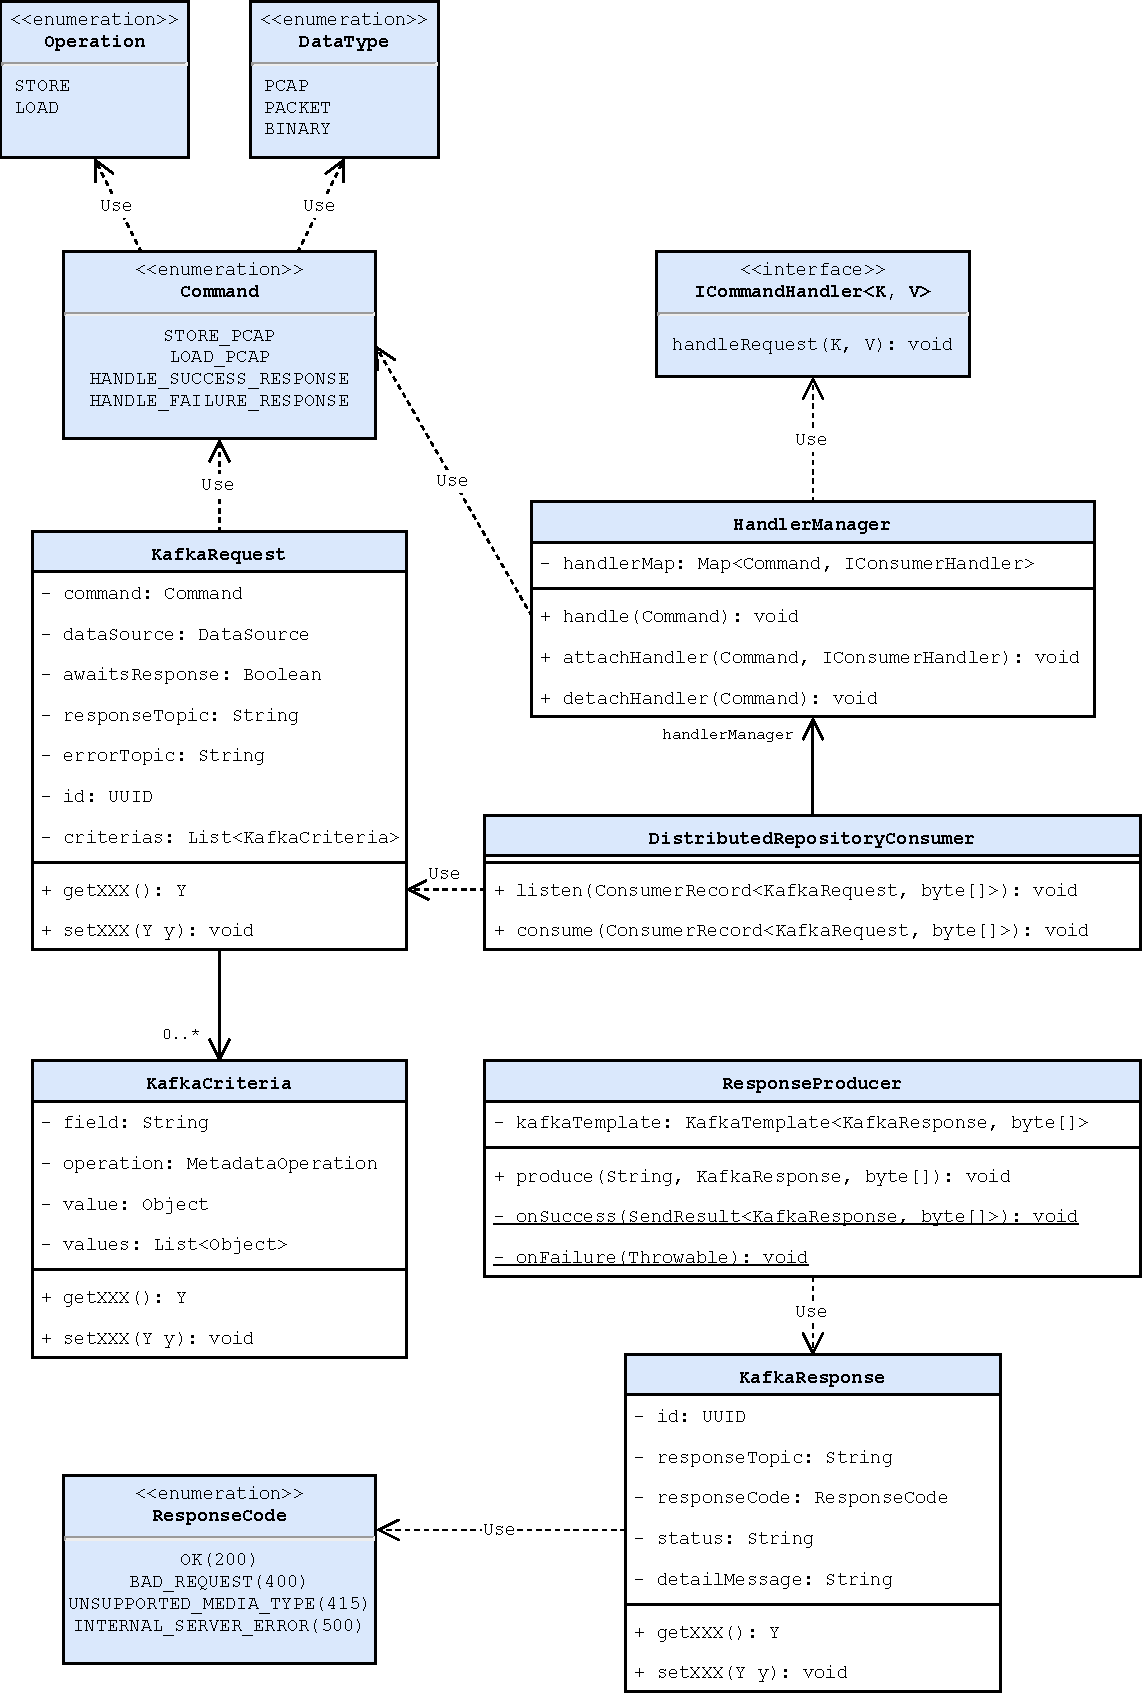
\includegraphics[width=15cm]{template-fig/CommunicationClassDiagram.pdf}
  \caption{Diagram tříd komunikace systému.}
  \label{FIG_CommunicationClassDiagram}
\end{figure}

\begin{figure}[!h]
  \centering
  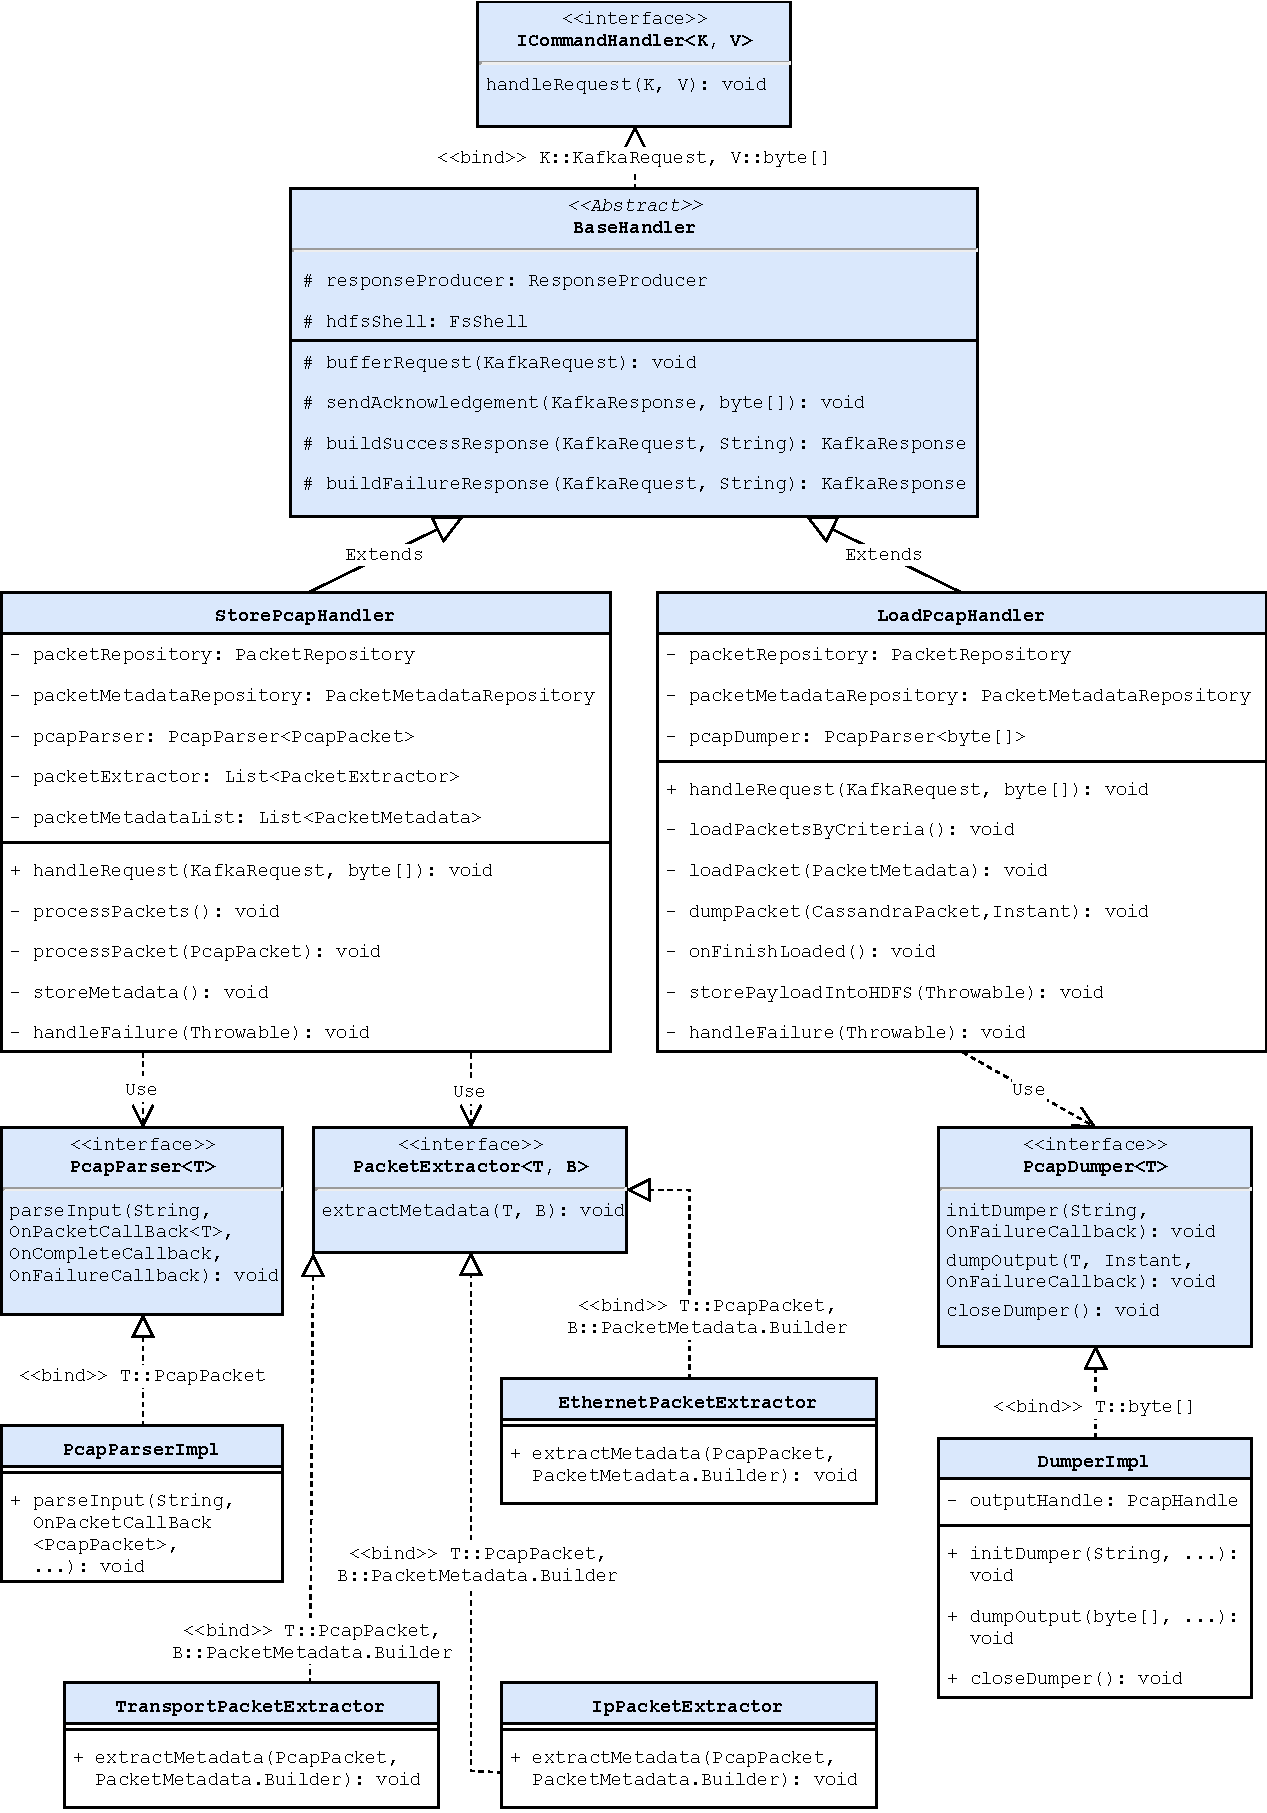
\includegraphics[width=15cm]{template-fig/DRCoreClassDiagram.pdf}
  \caption{Diagram tříd jádra systému.}
  \label{FIG_DRCoreClassDiagram}
\end{figure}

\subsection{Rozhraní pro dotazování dat} \label{queryDataInterface}
V~této sekci bude uvedeno jakým způsobem lze zadávat kritéria pro dotazování. Kritéria slouží k~filtrování záznamů, uplatní se na záznamy -- dokumenty metadat. Formát jednotlivých kritérií výrazně odpovídá tvaru parametrů dokumentů v~MongoDB.

Jeden objekt kritéria je reprezentován instancí třídy \texttt{KafkaCriteria} pocházející z~modulu Communication. Obsahuje tyto parametry:

\begin{itemize}
    \item \texttt{field} -- Řetězcová hodnota udávající název atributu v~dokumentu MongoDB.
    
    \item \texttt{operation} -- Jedná se o~hodnotu výčtu \texttt{MetadataOperation}, který obsahuje tyto názvy operací -- \texttt{is}, \texttt{ne}, \texttt{lt}, \texttt{lte}, \texttt{gt}, \texttt{gte}, \texttt{in}, \texttt{nin}. Tyto názvy porovnávacích operací reflektují názvy metod ve třídě \texttt{Criteria} z~modulu Spring Data, takže lze pomocí reflexe tento objekt sestavit. Způsob sestavení přes reflexi je zvolen kvůli chybějící závislosti modulu Persistence klientské aplikaci.
    Objekt \texttt{Criteria} lze potom předat do reaktivního dotazu do MongoDB.
    
    \item \texttt{value} -- Představuje hodnotu, podle které se atribut \texttt{field} bude filtrovat. Lze zadat libovolný Java objekt.
    
    \item \texttt{values} -- Operace \texttt{in} a~\texttt{nin} vyžadují seznam hodnot k~filtrování. K~předání seznamu objektů slouží tento parametr.
\end{itemize}

\noindent Objektů typu \texttt{KafkaCriteria} lze sestavit libovolné množství, a~předat je poté do zprávy požadavku \texttt{KafkaRequest} \ref{designCommunication}. Jednotlivé filtrovací operace se společně s~uvedenými atributy a~hodnotami zřetězí pomocí logické operace \texttt{and} do objektu třídy \texttt{Criteria}.

\subsection{Scénáře}
Tato sekce uvede podporované příkazy a~jakým způsobem jsou zpracovány. Podporovány jsou dva scénáře -- uložení PCAP souboru a~čtení paketů podle zadaných kritérií. Jádro distribuovaného repositáře ilustruje diagram tříd \ref{FIG_DRCoreClassDiagram}.

Zpracování proběhne následovně -- metoda \texttt{listen} třídy DistributedRepositoryConsumer zkonzumuje zprávu z~fronty a~zavolá metodu \texttt{consume}, která spustí obsluhu příkazu. Aktuálně jsou definovány dvě obsluhy:

\begin{itemize}
    \item Příkaz \texttt{STORE\_PCAP} - Zpracování řeší třída \texttt{StorePcapHandler}.
    \item Příkaz \texttt{LOAD\_PCAP} - Obsluhu poskytuje třída \texttt{LoadPcapHandler}. 
\end{itemize}

\subsubsection{Zpracování a~uložení PCAP souboru}
Klient odešle příkaz \texttt{STORE\_PCAP} s~dodatečnými parametry udávajícími zdroj dat a~výstupní frontu (více v~\ref{designCommunication}). Po přijetí zprávy požadavku proběhne uložení PCAP souboru do pomocného souboru na lokálním disku (z~HDFS a~nebo z~paměti RAM), protože knihovna Pcap4J neumí zpracovávat PCAP soubory z~HDFS ani z~paměti RAM. Následně proběhne parsování na jednotlivé pakety. K~tomu slouží rozhraní \texttt{PcapParser<T>} s~implementací dodanou ve třídě \texttt{PcapParserImpl}. Pakety jsou jeden po druhém ukládány do databáze Cassandra asynchronním způsobem \ref{cassandra}. Současně jsou také vytvářeny záznamy metadat. Extrahování informací z~paketů zajišťuje jednotné rozhraní \texttt{PacketExtractor<T, B>} s~několika implementacemi podle vrstev TCP/IP modelu -- \texttt{EthernetPacketExtractor}, \texttt{IpPacketExtractor} a~\texttt{TransportPacketExtractor}. Záznamy metadat se ukládají reaktivním způsobem \ref{mongoDB} po kolekcích obsahujících několik záznamů (počet záznamů, které se uloží najednou, lze konfigurovat pomocí položky \texttt{packet.metadata.max.list.size} \ref{configuration}). Až jsou všechny pakety i~záznamy metadat uloženy, lze odstranit dočasný PCAP soubor z~lokálního disku. Poté je případně odeslána odpověď klientovi s~návratovým kódem \texttt{OK(200)}.

\subsubsection{Čtení paketů podle kritérií}
Klient odešle příkaz \texttt{LOAD\_PCAP} s~dodatečnými parametry podobně jako v~předchozím případě. Navíc zadá dotazovací kritéria jejichž sémantika je uvedena v~\ref{queryDataInterface}. Po přijetí zprávy požadavku proběhne sestavení objektu \texttt{Criteria} z~kritérií uvedených ve zprávě požadavku. Tento objekt je předán do \texttt{packetMetadataRepository}, kde je pomocí Spring Data API provedeno čtení metadat paketů z~MongoDB. Čtení probíhá reaktivně se zabudovanými \texttt{callback}-y, které pro každý načtený záznam spustí další čtení, v~tomto případě už hodnoty celého paketu z~databáze Cassandra. Načítání paketů probíhá zase asynchronně, k~metodě je přidán další \texttt{callback}, který obslouží načtený paket tím, že jej zapíše do PCAP souboru (klient musí zadat cestu k~výslednému PCAP souboru pomocí atributu \texttt{dataSource} ve zprávě požadavku \ref{designCommunication}, předání souboru přes Kafku není možné z~důvodu neznámé velikosti a~počtu nalezených paketů). Přístup k~výslednému PCAP souboru je možný skrze rozhraní \texttt{PcapDumper<T>}, implementovaného ve třídě \texttt{DumperImpl}. PCAP soubor je až do konce čtení paketů uložen jako dočasný soubor (kvůli limitaci Pcap4J knihovny), potom je přesunut na HDFS. Celý proces končí odesláním odpovědi klientovi.

\subsection{Rozšíření pro nový typ forenzních dat}
Rozšíření v~podobě podpory nových druhů digitálních forenzních dat je velmi jednoduché. Spočívá v~přídání implementace:

\begin{itemize}
    \item Rozšíření výčtů \texttt{Command}, \texttt{Operation} a~\texttt{DataType}, kde lze přidat nové typy příkazů.
    
    \item Zpracování příkazu -- Je potřeba specializovat třídu \texttt{BaseHandler} novou implementací, která bude kompletně řídit zpracování příkazu (\texttt{BaseHandler} má přístup k~HDFS a~k~šabloně obsluhující komunikaci s~Kafkou). Tato implementace se musí nakonfigurovat jako bean ve třídě \texttt{HandlerBeans} a~asociovat s~typem příkazu přes správce handlerů v~\texttt{HandlerManagerBeans}.
\end{itemize}

\noindent Po těchto krocích lze zasílat zprávy požadavků s~novým typem příkazu z~klientské aplikace.

\section{Klientská aplikace}
Pro účely testování byla implementována i~klientská demo aplikace ProducerDemo \ref{FIG_Architecture}. 
Jedná se také o~aplikaci postavené na Spring Boot s~možností auto-konfigurace. Systém podporuje zaslání zpráv požadavků pro dva výše zmíněné scénáře -- požadavek pro uložení PCAP souboru, a~požadavek pro čtení paketů podle kritérií. Data předává v~obou případech přes HDFS z~důvodu šetření paměti RAM. Odpovědi z~distribuovaného úložiště přijímají dvě rozdílné komponenty:

\begin{itemize}
    \item \texttt{AcknowledgementConsumerHandler} -- Přijímá zprávy pouze z~výstupní Kafka fronty \texttt{output\_topic}.
    
    \item \texttt{ErrorConsumerHandler} -- Přijímá zprávy z~chybové fronty \texttt{error\_topic}.
\end{itemize}

\noindent Čtení zpráv z~těchto dvou front je rozděleno do různých tříd pro potenciálně lepší zpracování chyb. Aktuálně jsou všechny příchozí odpovědi (v~obou třídách) zapsány do logů.

Příklady spuštění aplikací jsou uvedeny v~\ref{launching}.

\section{Logování}
Logování (angl. \texttt{logging}) pomáhá trasování běžícího systému. Existuje mnoho implementací pro trasování v~Java (\texttt{Log4j}, \texttt{Log4j 2}, \texttt{Logback} atd.). Konkrétní implementaci už v~sobě jako závislost zahrnuje přímo Spring Boot. Logování lze konfigurovat mnoha parametry. Lze určit, do kterého souboru se bude zapisovat, jakou úroveň logování použít, formát zapisovaných zpráv, nastavení se může lišit pro jednotlivé balíčky apod. Každá implementace logovacího systému by měla podporovat následující úrovně logování -- \texttt{TRACE}, \texttt{DEBUG}, \texttt{INFO}, \texttt{WARN}, \texttt{ERROR}, \texttt{OFF}. Jednotlivé úrovně potom vyjadřují význam zprávy v~logu. Odpovídající nastavení v~systému distribuovaného úložiště lze vidět v~\ref{configuration}.

\section{Zpracování chyb}
Při běhu systému může nastat několik druhů chyb -- nefungující připojení k~databázi, pokud databáze neběží korektně; nedostupnost Kafka front; chyby při ukládání souborů na HDFS např. kvůli kolizi jmen nebo nedostatečnému oprávnění; chyby při parsování PCAP souboru či zápisu do PCAP souboru. Výjimky jsou odchyceny v~blocích \texttt{try} a~\texttt{catch}, v~případě reaktivních či asynchronních dotazů jsou zaregistrovány odpovídající \texttt{callback}-y pro chybové stavy. Po odchycení výjimek jsou výjimky logovány s~úrovní \texttt{ERROR}. Poté je sestavena odpověď pro klienta s~návratovým kódem \texttt{INTERNAL\_SERVER\_ERROR(500)} a~odpověď odeslána do chybové fronty zadané parametrem \texttt{errorTopic} uvedeného ve zprávě požadavku.

\chapter{Výkon} \label{chapter_performance}

\chapter{Závěr}

\section{Výsledky}
V~rámci teoretické části práce jsem se seznámil s~forenzní analýzou digitálních dat. Prozkoumal jsem existující systémy pro uložení digitálních forenzních dat (včetně AFF4). Seznámil jsem se s~distribuovanými databázemi a~NoSQL databázemi.

Navrhl jsem distribuované úložiště rozsáhlých digitálních forenzních dat včetně aplikačního rozhraní, a~vybral vhodné technologie pro realizaci.

Implementovaný systém řeší požadované aspekty, je založen na distribuovaných technologiích počítajících se škálovatelností. Architektura umožňuje přidat podporu pro nové druhy forenzních dat. S~pomocí Spring Boot a~ostatních Spring projektů je jednoduchá konfigurace celého systému. Detaily k~běhovému prostředí implementovaných aplikací jsou uvedeny v~\ref{dockerEnv}.

\vspace{0.5cm}
\noindent \textbf{TODO: Vyhodnocení výkonu}

\section{Navržená rozšíření}

%=========================================================================
 % viz. obsah.tex / see obsah.tex

  % Pouzita literatura / Bibliography
  % ----------------------------------------------
\ifslovak
  \makeatletter
  \def\@openbib@code{\addcontentsline{toc}{chapter}{Literatúra}}
  \makeatother
  \bibliographystyle{bib-styles/czechiso}
\else
  \ifczech
    \makeatletter
    \def\@openbib@code{\addcontentsline{toc}{chapter}{Literatura}}
    \makeatother
    \bibliographystyle{bib-styles/czechiso}
  \else 
    \makeatletter
    \def\@openbib@code{\addcontentsline{toc}{chapter}{Bibliography}}
    \makeatother
    \bibliographystyle{bib-styles/englishiso}
  %  \bibliographystyle{alpha}
  \fi
\fi
  \begin{flushleft}
  \bibliography{projekt-20-literatura-bibliography}
  \end{flushleft}

  % vynechani stranky v oboustrannem rezimu
  % Skip the page in the two-sided mode
  \iftwoside
    \cleardoublepage
  \fi

  % Prilohy / Appendices
  % ---------------------------------------------
  \appendix
\ifczech
  \renewcommand{\appendixpagename}{Přílohy}
  \renewcommand{\appendixtocname}{Přílohy}
  \renewcommand{\appendixname}{Příloha}
\fi
\ifslovak
  \renewcommand{\appendixpagename}{Prílohy}
  \renewcommand{\appendixtocname}{Prílohy}
  \renewcommand{\appendixname}{Príloha}
\fi
%  \appendixpage

% vynechani stranky v oboustrannem rezimu
% Skip the page in the two-sided mode
%\iftwoside
%  \cleardoublepage
%\fi
  
\ifslovak
%  \section*{Zoznam príloh}
%  \addcontentsline{toc}{section}{Zoznam príloh}
\else
  \ifczech
%    \section*{Seznam příloh}
%    \addcontentsline{toc}{section}{Seznam příloh}
  \else
%    \section*{List of Appendices}
%    \addcontentsline{toc}{section}{List of Appendices}
  \fi
\fi
  \startcontents[chapters]
  \setlength{\parskip}{0pt}
  % seznam příloh / list of appendices
  % \printcontents[chapters]{l}{0}{\setcounter{tocdepth}{2}}
  
  \ifODSAZ
    \setlength{\parskip}{0.5\bigskipamount}
  \else
    \setlength{\parskip}{0pt}
  \fi
  
  % vynechani stranky v oboustrannem rezimu
  \iftwoside
    \cleardoublepage
  \fi
  % Tento soubor nahraďte vlastním souborem s přílohami (nadpisy níže jsou pouze pro příklad)
% This file should be replaced with your file with an appendices (headings below are examples only)

% Umístění obsahu paměťového média do příloh je vhodné konzultovat s vedoucím
% Placing of table of contents of the memory media here should be consulted with a supervisor
%\chapter{Obsah přiloženého paměťového média}

%\chapter{Manuál}

\chapter{Konfigurace} \label{configuration}
\section{Systém distribuovaného úložiště}
Konfigurace aplikace DistributedRepository se nachází v~souboru \\ \texttt{DistributedRepository/src/main/resources/application.properties} \\
a~obsahuje tyto položky:

\vspace{0.5cm}
\noindent \texttt{\#   Cassandra \\
spring.data.cassandra.keyspace-name=structured\_data \\
spring.data.cassandra.contact-points=192.168.99.100 \\
spring.data.cassandra.port=9042 \\
\#   Hadoop \\
spring.hadoop.fs-uri=hdfs://172.17.0.4:9000 \\
\#   Kafka \\
spring.kafka.bootstrap-servers=192.168.99.100:9092 \\
spring.kafka.consumer.auto-commit-interval=1000 \\
spring.kafka.consumer.enable-auto-commit=true \\
spring.kafka.consumer.group-id=test \\
spring.kafka.consumer.key-deserializer= \\
\indent cz.vutbr.fit.communication.serialization.KafkaRequestDeserializer \\
spring.kafka.consumer.value-deserializer= \\
\indent org.apache.kafka.common.serialization.ByteArrayDeserializer \\
spring.kafka.producer.acks=all \\
spring.kafka.producer.batch-size=16384 \\
spring.kafka.producer.bootstrap-servers=192.168.99.100:9092 \\
spring.kafka.producer.buffer-memory=335544320 \\
spring.kafka.producer.key-serializer= \\
\indent cz.vutbr.fit.communication.serialization.KafkaResponseSerializer \\
spring.kafka.producer.properties.max.request.size=500000000 \\
spring.kafka.producer.retries=0 \\
spring.kafka.producer.value-serializer= \\
\indent org.apache.kafka.common.serialization.ByteArraySerializer \\
input.topic=input\_topic \\
output.topic=output\_topic \\
error.topic=error\_topic \\
\#   Logging \\
logging.level.cz.vutbr.fit=DEBUG \\
logging.level.org.pcap4j.core=INFO \\
\#   MongoDB \\
spring.data.mongodb.host=192.168.99.100 \\
spring.data.mongodb.port=27017 \\
spring.data.mongodb.database=metadata \\
\#   StorePcapHandler \\
packet.metadata.max.list.size=500 \\
tmp.directory=tmp/
}

\section{Klientská aplikace}
Konfigurace aplikace ProducerDemo se nachází v~souboru \\
\texttt{ProducerDemo/src/main/resources/application.properties} \\
a~obsahuje tyto položky:

\vspace{0.5cm}
\noindent \texttt{\#   Hadoop \\
spring.hadoop.fs-uri=hdfs://172.17.0.4:9000 \\
\#   Kafka \\
spring.kafka.bootstrap-servers=192.168.99.100:9092 \\
spring.kafka.consumer.auto-commit-interval=1000 \\
spring.kafka.consumer.enable-auto-commit=true \\
spring.kafka.consumer.group-id=test \\
spring.kafka.consumer.key-deserializer= \\
\indent cz.vutbr.fit.communication.serialization.KafkaResponseDeserializer \\
spring.kafka.consumer.value-deserializer= \\
\indent org.apache.kafka.common.serialization.ByteArrayDeserializer \\
spring.kafka.producer.acks=all \\
spring.kafka.producer.batch-size=16384 \\
spring.kafka.producer.bootstrap-servers=192.168.99.100:9092 \\
spring.kafka.producer.buffer-memory=335544320 \\
spring.kafka.producer.key-serializer= \\
\indent cz.vutbr.fit.communication.serialization.KafkaRequestSerializer \\
spring.kafka.producer.properties.max.request.size=500000000 \\
spring.kafka.producer.retries=0 \\
spring.kafka.producer.value-serializer= \\
\indent org.apache.kafka.common.serialization.ByteArraySerializer \\
input.topic=input\_topic \\
output.topic=output\_topic \\
error.topic=error\_topic \\
\#   Logging \\
logging.level.cz.vutbr.fit=DEBUG \\
\#   StorePcapProducerDemo \\
cz.vutbr.fit.producerdemo.demo.StorePcapProducerDemo.dataSourceStorage=HDFS \\
\#   LoadPcapProducerDemo \\
cz.vutbr.fit.producerdemo.demo.LoadPcapProducerDemo.dataSourceStorage=HDFS
}

\chapter{Běhové prostředí} \label{dockerEnv}
Jako běhové prostředí pro systém distribuovaného repositáře byl zvolen projekt \texttt{Docker} \footnote{https://www.docker.com/} z~důvodu jednodušší a~oddělené správy použitých technologií. Každá technologie běží v~odděleném kontejneru spuštěném z~předem připraveného obrazu. Všechny soubory a~skripty týkající se běhového prostředí jsou uloženy v~adresáři \texttt{Docker/}.

\section{Obrazy}
Každou technologii reprezentuje samostatný obraz (angl. \texttt{image}), v~němž je daná technologie nainstalována.

\vspace{0.5cm}
\noindent Kompletní přehled obrazů:

\begin{lstlisting}[language=bash,basicstyle={\small\ttfamily}]
$ docker image ls
REPOSITORY                  TAG                 IMAGE ID         CREATED          SIZE
martinfit/maven             3.5.2-jdk-9-slim    b78e23733813     3 hours ago      449MB
martinfit/cassandra         3                   9a1473c2fc55     3 hours ago      323MB
wurstmeister/kafka          1.0.1               2e0c23534746     2 weeks ago      330MB
mongo                       3.4                 9ad59b0c0624     3 weeks ago      360MB
cassandra                   3                   c6b513da2ff3     4 weeks ago      323MB
maven                       3.5.2-jdk-9-slim    58405637ffbb     8 weeks ago      392MB
wurstmeister/zookeeper      latest              351aa00d2fe9     16 months ago    478MB
sequenceiq/hadoop-docker    2.7.1               42efa33d1fa3     2 years ago      1.76GB
\end{lstlisting}

\noindent Většina výše uvedených obrazů pochází přímo z~oficiálního repositáře \texttt{Docker Hub} \footnote{https://hub.docker.com/}. Výjimku tvoří obrazy \texttt{martinfit/maven} a~\texttt{martinfit/cassandra}. Tyto dva obrazy jsou založeny na obrazech z~Docker Hub, ale byla do nich přidána dodatečná konfigurace. Obraz pro databázi Cassandra byl mírně upraven, aby bylo možné inicializovat schéma databáze při spuštění kontejneru. Do obrazu pro nástroj Maven byla doinstalována nativní knihovna \texttt{libpcap} kvůli korektnímu běhu knihovny Pcap4J \ref{pcap4j}.

Instalaci prostředí (tzn. stažení a~sestavení obrazů) provádí nástroje \texttt{docker-compose pull} a~\texttt{docker build} uvnitř skriptu \texttt{install-docker-enviroment.sh}. Spuštění kontejnerů z~definovaných obrazů zajistí skript \texttt{run-docker-enviroment.sh}. Zastavit kontejnery lze pomocí skriptu \texttt{stop-docker-enviroment.sh}. Veškerá konfigurace obrazů a~kontejnerů se nachází v~souboru \texttt{Environment/docker-compose.yml}.

\chapter{Spuštění aplikací} \label{launching}
Sestavení jednotlivých modulů zajišťují přiložené skripty \texttt{install.sh} v~adresáři každého modulu. Jednotlivé cesty ke skriptům jsou:

\begin{enumerate}
    \item \texttt{Communication/install.sh}
    
    \item \texttt{Persistence/install.sh}
    
    \item \texttt{DistributedRepository/install.sh}
    
    \item \texttt{ProducerDemo/install.sh}
\end{enumerate}

\noindent Kvůli závislostem mezi moduly je nutné skripty spustit ve výše uvedeném pořadí. Moduly jsou zkompilovány a~sestaveny pomocí nástroje Maven, který provede stažení všech potřebných závislostí.

\section{DistributedRepository}
Systém distribuovaného úložiště lze spustit skriptem \texttt{DistributedRepository/run.sh}, který dynamicky zjistí IP adresy běžících kontejnerů v~Docker, a~na základě zjištěných hodnot přepíše aplikační proměnné.

\section{ProducerDemo}
Klientskou aplikaci lze spustit pomocí skriptu \texttt{ProducerDemo/run.sh}, který také dynamicky přepíše aplikační proměnné podle běžících kontejnerů.

\chapter{Data měření výkonnosti}

\section{Prototyp}

\begin{table}[h!]
    \centering
    \begin{tabular}{| l | l | l | l | l |}
    \hline
    \texttt{PCAP size (B)}   &   \texttt{Count of packets}   &   \texttt{Avg. packet size} &  \texttt{Time (s)} &   \texttt{Packets/s} \\ \hline
    91 340 & 382 & 239,1099476 & 7 & 54,57142857 \\ \hline
    1 955 172 & 1360 & 1437,626471 & 13 & 104,6153846 \\ \hline
    412 254 & 1879 & 219,4007451 & 19 & 98,89473684 \\ \hline
    420 869 & 2263 & 185,9783473 & 23 & 98,39130435 \\ \hline
    449 234 & 2563 & 175,276629 & 29 & 88,37931034 \\ \hline
    \end{tabular}\par
    \bigskip
    \caption{Tabulka obsahuje data naměřená při testování výkonnosti prototypu.}
    \label{tablePerformancePrototype}
\end{table}

\section{Finální systém}

\begin{table}[h!]
    \centering
    \begin{tabular}{| l | l | l | l | l |}
    \hline
    \texttt{PCAP size (B)}   &   \texttt{Count of packets}   &   \texttt{Avg. packet size} &  \texttt{Time (s)} &   \texttt{Packets/s} \\ \hline
    91 340 & 382 & 239,1099476 & 0,5 & 764 \\ \hline
    1 955 172 & 1360 & 1437,626471 & 0,5 & 2720 \\ \hline
    412 254 & 1879 & 219,4007451 & 0,5 & 3758 \\ \hline
    420 869 & 2263 & 185,9783473 & 1 & 2263 \\ \hline
    449 234 & 2563 & 175,276629 & 1,5 & 1709 \\ \hline
    \end{tabular}\par
    \bigskip
    \caption{Tabulka obsahuje data naměřená při testování výkonnosti finálního systému.}
    \label{tablePerformanceFinalSystem}
\end{table}

%\chapter{Plakát} % poster
 % viz. prilohy.tex / see prilohy.tex
\end{document}
